\documentclass[11pt]{article}
\usepackage[textwidth=18.0cm, textheight=23.0cm, top=2.0cm]{geometry}
\usepackage{pst-all}
\usepackage{amssymb}
\usepackage{tikz}
\usepackage{underscore}\begin{document}
\pagestyle{empty}


ClassName: \underline{\textbf{Class_03.2bp-45}}
\par
BinSize: \underline{\textbf{40 × 40}}
\par
ReduceSize: \underline{\textbf{40 × 40}}
\par
TypeNum: \underline{\textbf{99}}
\par
Num: \underline{\textbf{100}}
\par
OutS: \underline{\textbf{43200}}
\par
InS: \underline{\textbf{36761}}
\par
Rate: \underline{\textbf{0.851}}
\par
UB: \underline{\textbf{27}}
\par
LB0: \underline{\textbf{27}}
\par
LB: \underline{\textbf{27}}
\par
LBWithCut: \underline{\textbf{27}}
\par
NodeCut: \underline{\textbf{0}}
\par
ExtendedNodeCnt: \underline{\textbf{1}}
\par
GenNodeCnt: \underline{\textbf{1}}
\par
PrimalNode: \underline{\textbf{0}}
\par
ColumnCount: \underline{\textbf{27}}
\par
TotalCutCount: \underline{\textbf{0}}
\par
RootCutCount: \underline{\textbf{0}}
\par
LPSolverCnt: \underline{\textbf{1}}
\par
PricingSolverCnt: \underline{\textbf{0}}
\par
BranchAndBoundNum: \underline{\textbf{1}}
\par
isOpt: \underline{\textbf{true}}
\par
TimeOnInitSolution: \underline{\textbf{0.020 s}}
\par
TimeOnPrimal: \underline{\textbf{0.000 s}}
\par
TimeOnPricing: \underline{\textbf{0.000 s}}
\par
TimeOnRmp: \underline{\textbf{0.078 s}}
\par
TotalTime: \underline{\textbf{0.161 s}}
\par
\newpage


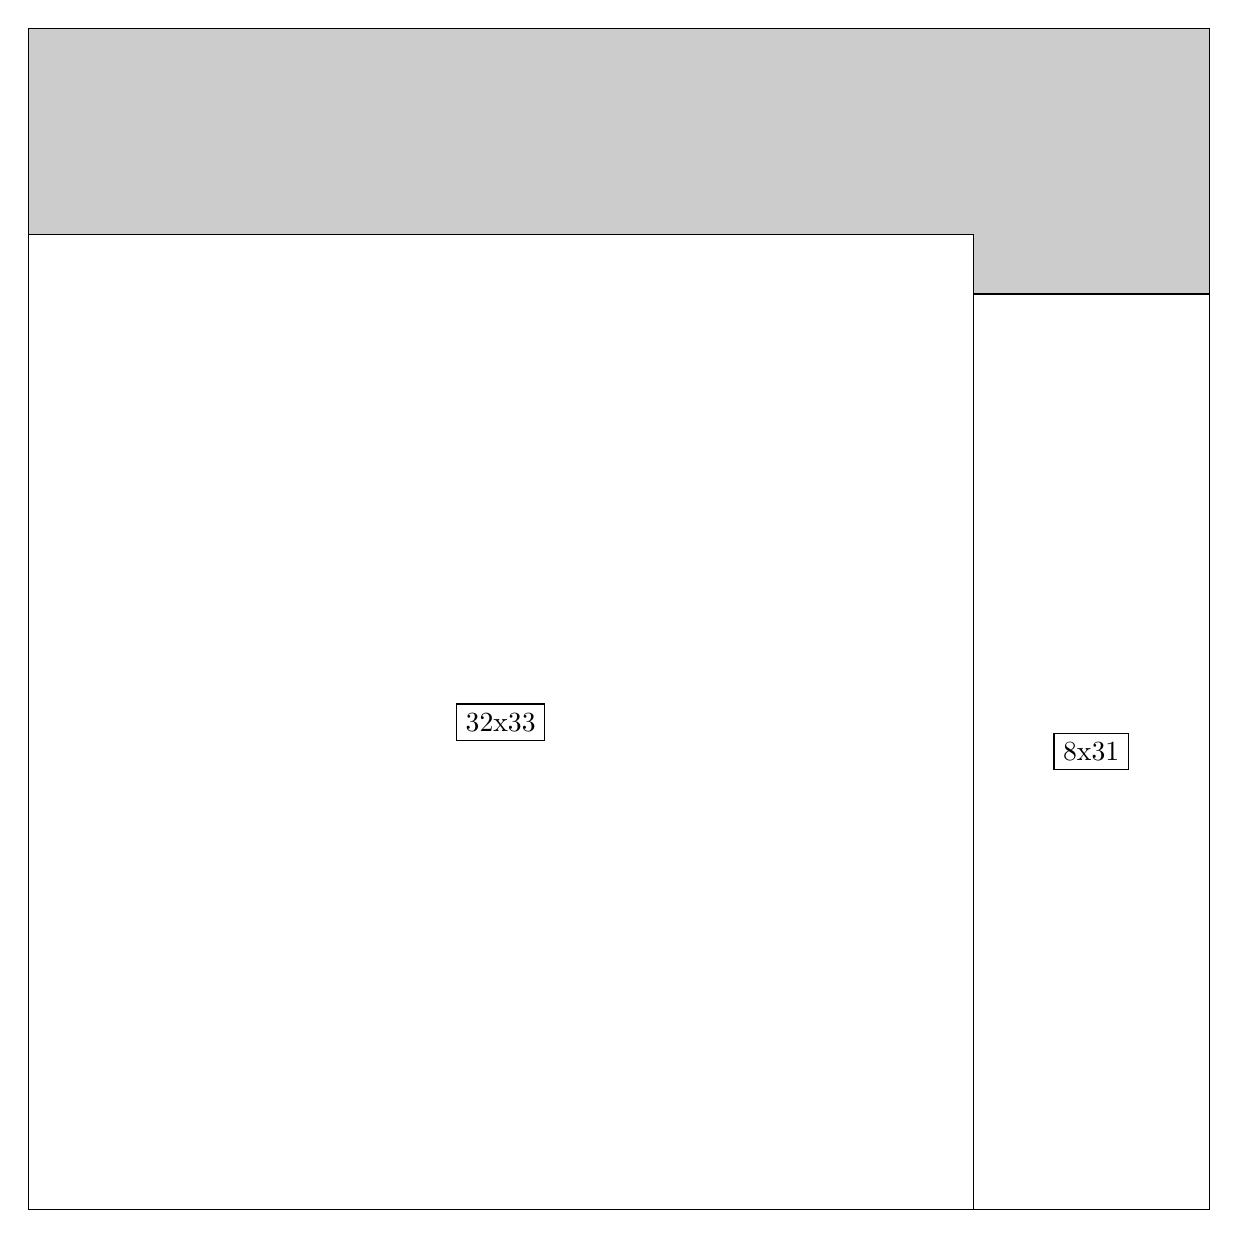
\begin{tikzpicture}[shorten >=1pt,scale=1.0,every node/.style={scale=1.0},->]
\tikzstyle{vertex}=[circle,fill=black!25,minimum size=14pt,inner sep=0pt]
\filldraw[fill=gray!40!white, draw=black] (0,0) rectangle (15.0,15.0);
\foreach \name/\x/\y/\w/\h in {32x33/0.0/0.0/12.0/12.375,8x31/12.0/0.0/3.0/11.625}
\filldraw[fill=white!40!white, draw=black] (\x,\y) rectangle node[draw] (\name) {\name} ++(\w,\h);
\end{tikzpicture}


w =32 , h =33 , x =0 , y =0 , v =1056
\par
w =8 , h =31 , x =32 , y =0 , v =248
\par
\newpage


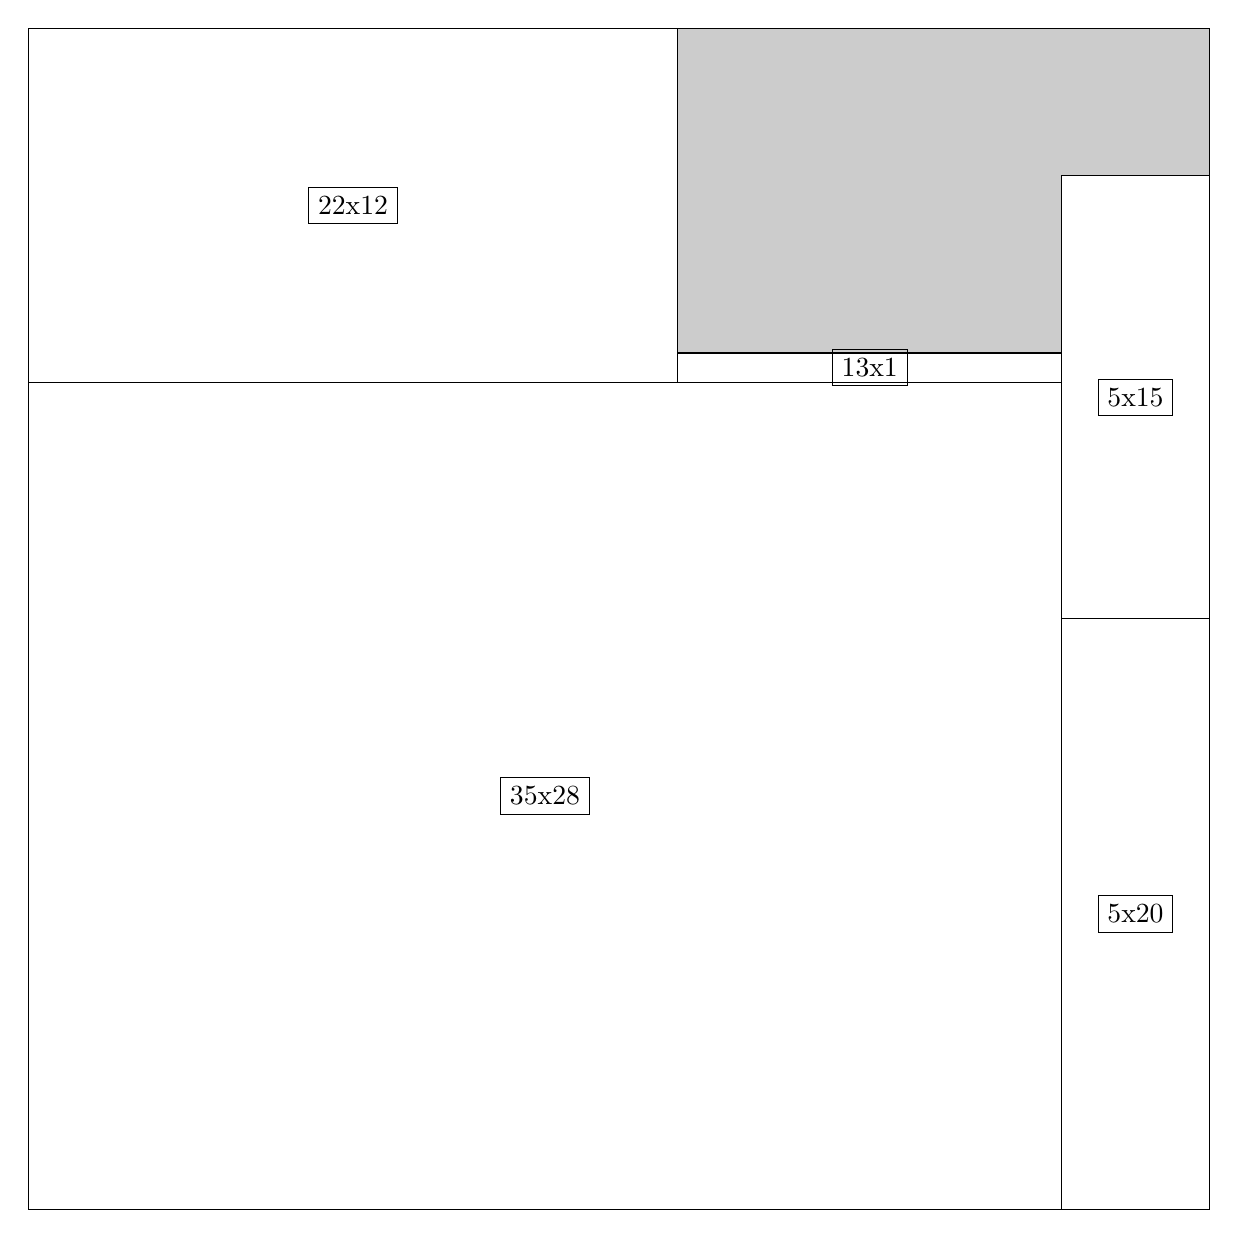
\begin{tikzpicture}[shorten >=1pt,scale=1.0,every node/.style={scale=1.0},->]
\tikzstyle{vertex}=[circle,fill=black!25,minimum size=14pt,inner sep=0pt]
\filldraw[fill=gray!40!white, draw=black] (0,0) rectangle (15.0,15.0);
\foreach \name/\x/\y/\w/\h in {35x28/0.0/0.0/13.125/10.5,22x12/0.0/10.5/8.25/4.5,5x20/13.125/0.0/1.875/7.5,5x15/13.125/7.5/1.875/5.625,13x1/8.25/10.5/4.875/0.375}
\filldraw[fill=white!40!white, draw=black] (\x,\y) rectangle node[draw] (\name) {\name} ++(\w,\h);
\end{tikzpicture}


w =35 , h =28 , x =0 , y =0 , v =980
\par
w =22 , h =12 , x =0 , y =28 , v =264
\par
w =5 , h =20 , x =35 , y =0 , v =100
\par
w =5 , h =15 , x =35 , y =20 , v =75
\par
w =13 , h =1 , x =22 , y =28 , v =13
\par
\newpage


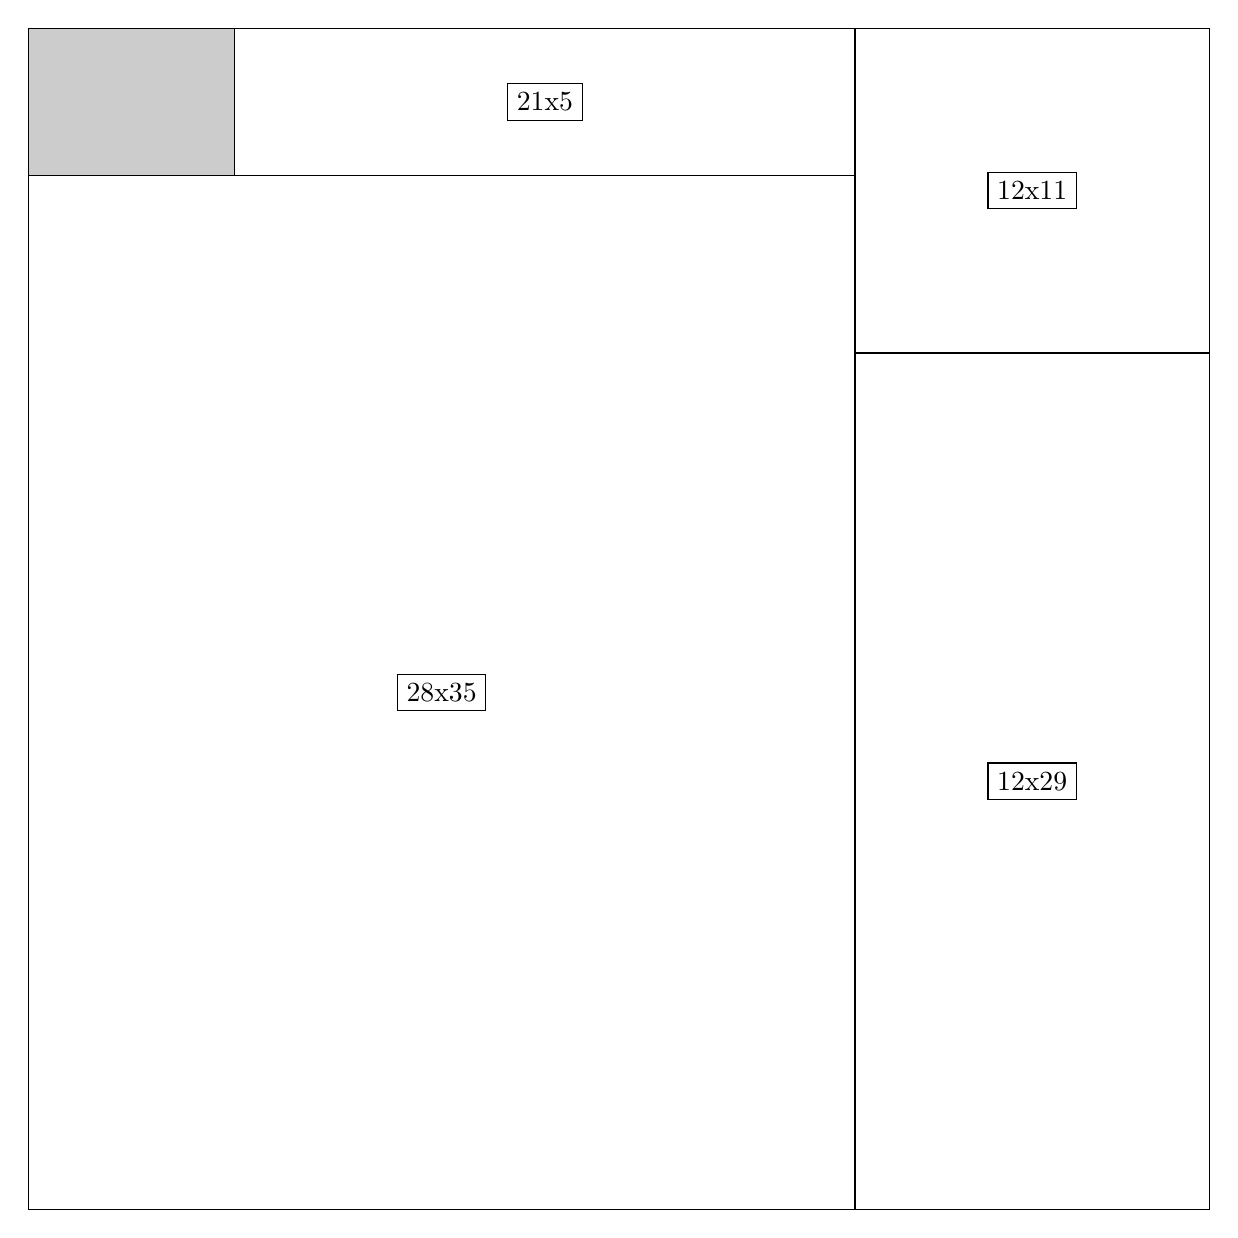
\begin{tikzpicture}[shorten >=1pt,scale=1.0,every node/.style={scale=1.0},->]
\tikzstyle{vertex}=[circle,fill=black!25,minimum size=14pt,inner sep=0pt]
\filldraw[fill=gray!40!white, draw=black] (0,0) rectangle (15.0,15.0);
\foreach \name/\x/\y/\w/\h in {28x35/0.0/0.0/10.5/13.125,12x29/10.5/0.0/4.5/10.875,12x11/10.5/10.875/4.5/4.125,21x5/2.625/13.125/7.875/1.875}
\filldraw[fill=white!40!white, draw=black] (\x,\y) rectangle node[draw] (\name) {\name} ++(\w,\h);
\end{tikzpicture}


w =28 , h =35 , x =0 , y =0 , v =980
\par
w =12 , h =29 , x =28 , y =0 , v =348
\par
w =12 , h =11 , x =28 , y =29 , v =132
\par
w =21 , h =5 , x =7 , y =35 , v =105
\par
\newpage


\begin{tikzpicture}[shorten >=1pt,scale=1.0,every node/.style={scale=1.0},->]
\tikzstyle{vertex}=[circle,fill=black!25,minimum size=14pt,inner sep=0pt]
\filldraw[fill=gray!40!white, draw=black] (0,0) rectangle (15.0,15.0);
\foreach \name/\x/\y/\w/\h in {34x28/0.0/0.0/12.75/10.5,34x10/0.0/10.5/12.75/3.75,6x34/12.75/0.0/2.25/12.75,22x2/6.75/14.25/8.25/0.75,14x2/1.5/14.25/5.25/0.75,6x4/12.75/12.75/2.25/1.5}
\filldraw[fill=white!40!white, draw=black] (\x,\y) rectangle node[draw] (\name) {\name} ++(\w,\h);
\end{tikzpicture}


w =34 , h =28 , x =0 , y =0 , v =952
\par
w =34 , h =10 , x =0 , y =28 , v =340
\par
w =6 , h =34 , x =34 , y =0 , v =204
\par
w =22 , h =2 , x =18 , y =38 , v =44
\par
w =14 , h =2 , x =4 , y =38 , v =28
\par
w =6 , h =4 , x =34 , y =34 , v =24
\par
\newpage


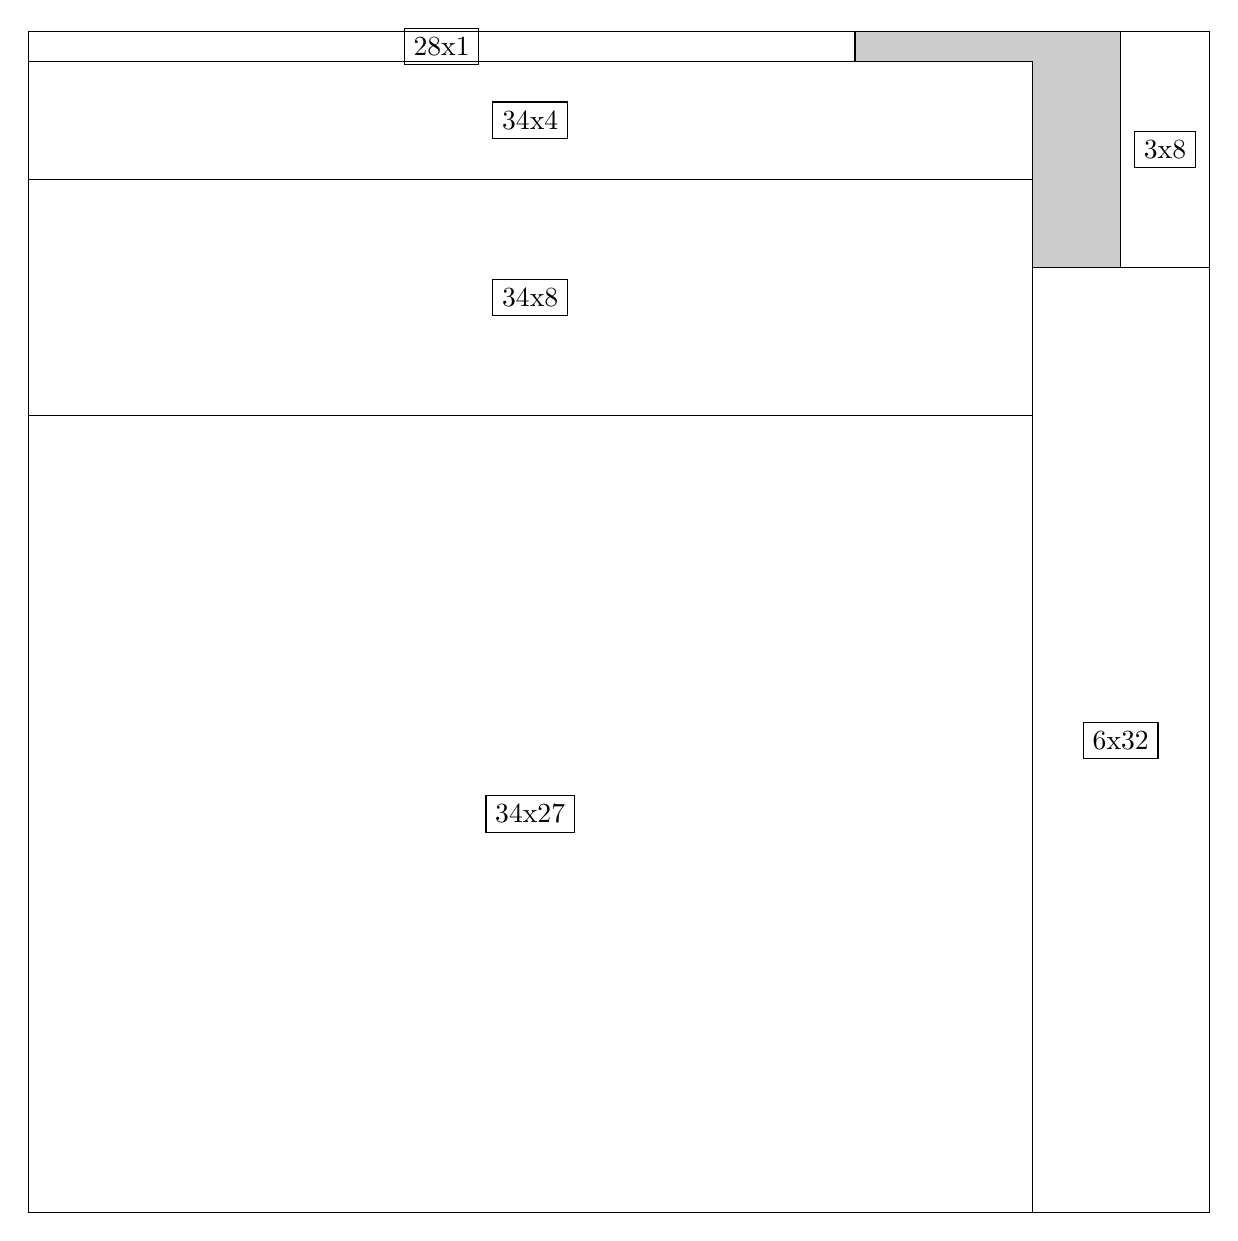
\begin{tikzpicture}[shorten >=1pt,scale=1.0,every node/.style={scale=1.0},->]
\tikzstyle{vertex}=[circle,fill=black!25,minimum size=14pt,inner sep=0pt]
\filldraw[fill=gray!40!white, draw=black] (0,0) rectangle (15.0,15.0);
\foreach \name/\x/\y/\w/\h in {34x27/0.0/0.0/12.75/10.125,34x8/0.0/10.125/12.75/3.0,6x32/12.75/0.0/2.25/12.0,34x4/0.0/13.125/12.75/1.5,28x1/0.0/14.625/10.5/0.375,3x8/13.875/12.0/1.125/3.0}
\filldraw[fill=white!40!white, draw=black] (\x,\y) rectangle node[draw] (\name) {\name} ++(\w,\h);
\end{tikzpicture}


w =34 , h =27 , x =0 , y =0 , v =918
\par
w =34 , h =8 , x =0 , y =27 , v =272
\par
w =6 , h =32 , x =34 , y =0 , v =192
\par
w =34 , h =4 , x =0 , y =35 , v =136
\par
w =28 , h =1 , x =0 , y =39 , v =28
\par
w =3 , h =8 , x =37 , y =32 , v =24
\par
\newpage


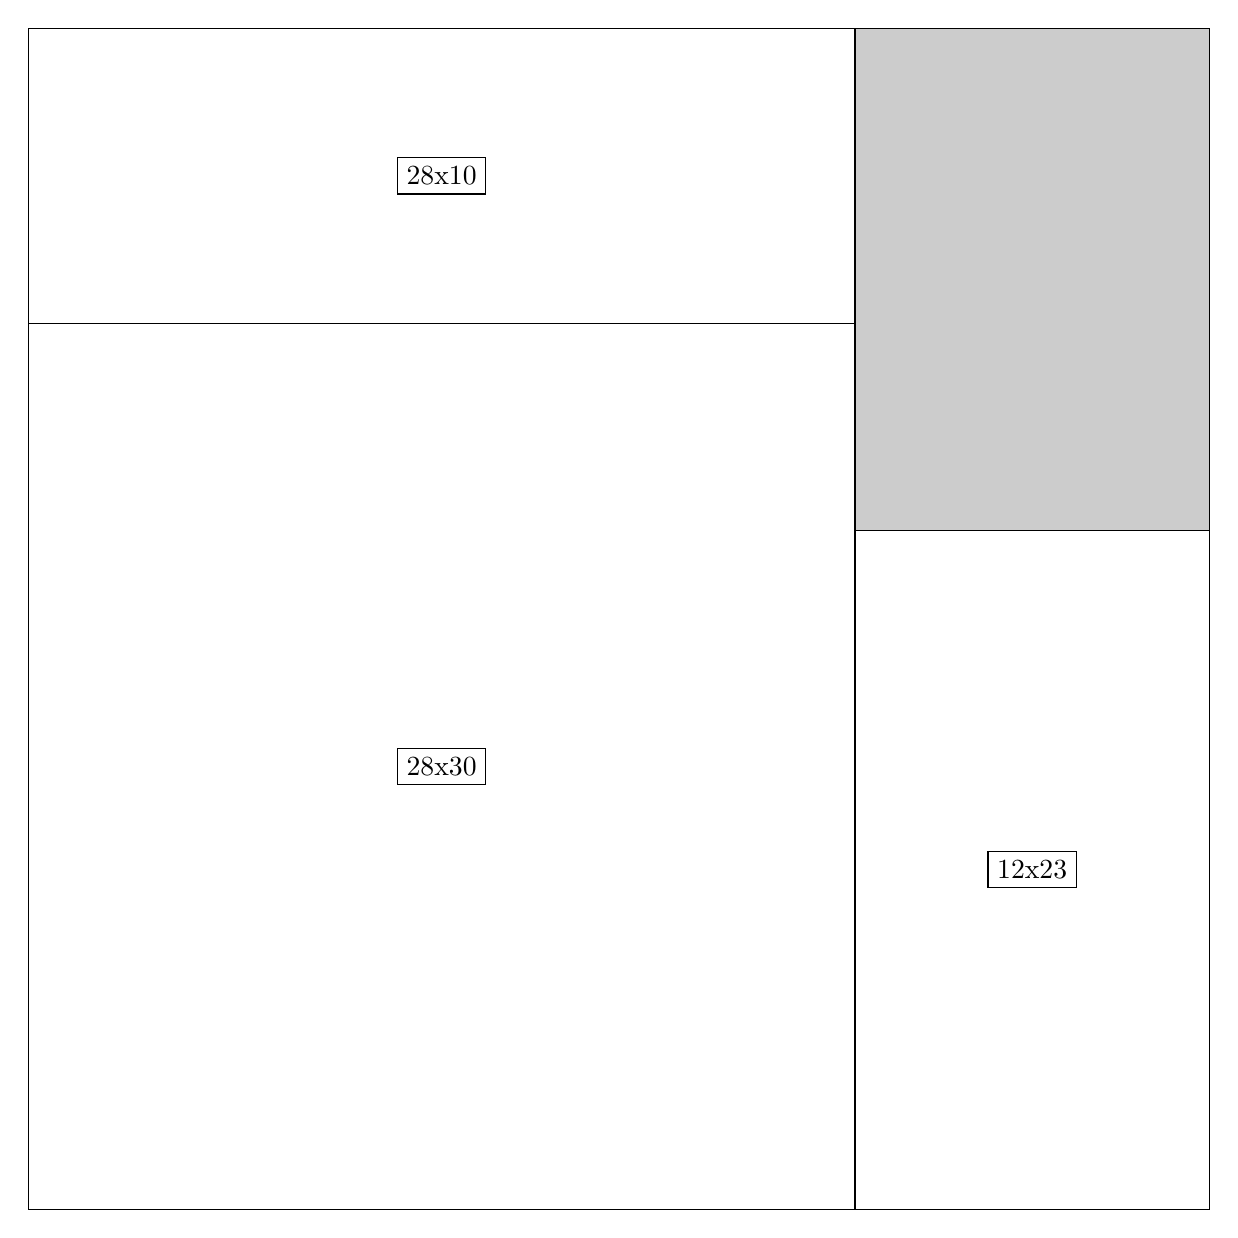
\begin{tikzpicture}[shorten >=1pt,scale=1.0,every node/.style={scale=1.0},->]
\tikzstyle{vertex}=[circle,fill=black!25,minimum size=14pt,inner sep=0pt]
\filldraw[fill=gray!40!white, draw=black] (0,0) rectangle (15.0,15.0);
\foreach \name/\x/\y/\w/\h in {28x30/0.0/0.0/10.5/11.25,28x10/0.0/11.25/10.5/3.75,12x23/10.5/0.0/4.5/8.625}
\filldraw[fill=white!40!white, draw=black] (\x,\y) rectangle node[draw] (\name) {\name} ++(\w,\h);
\end{tikzpicture}


w =28 , h =30 , x =0 , y =0 , v =840
\par
w =28 , h =10 , x =0 , y =30 , v =280
\par
w =12 , h =23 , x =28 , y =0 , v =276
\par
\newpage


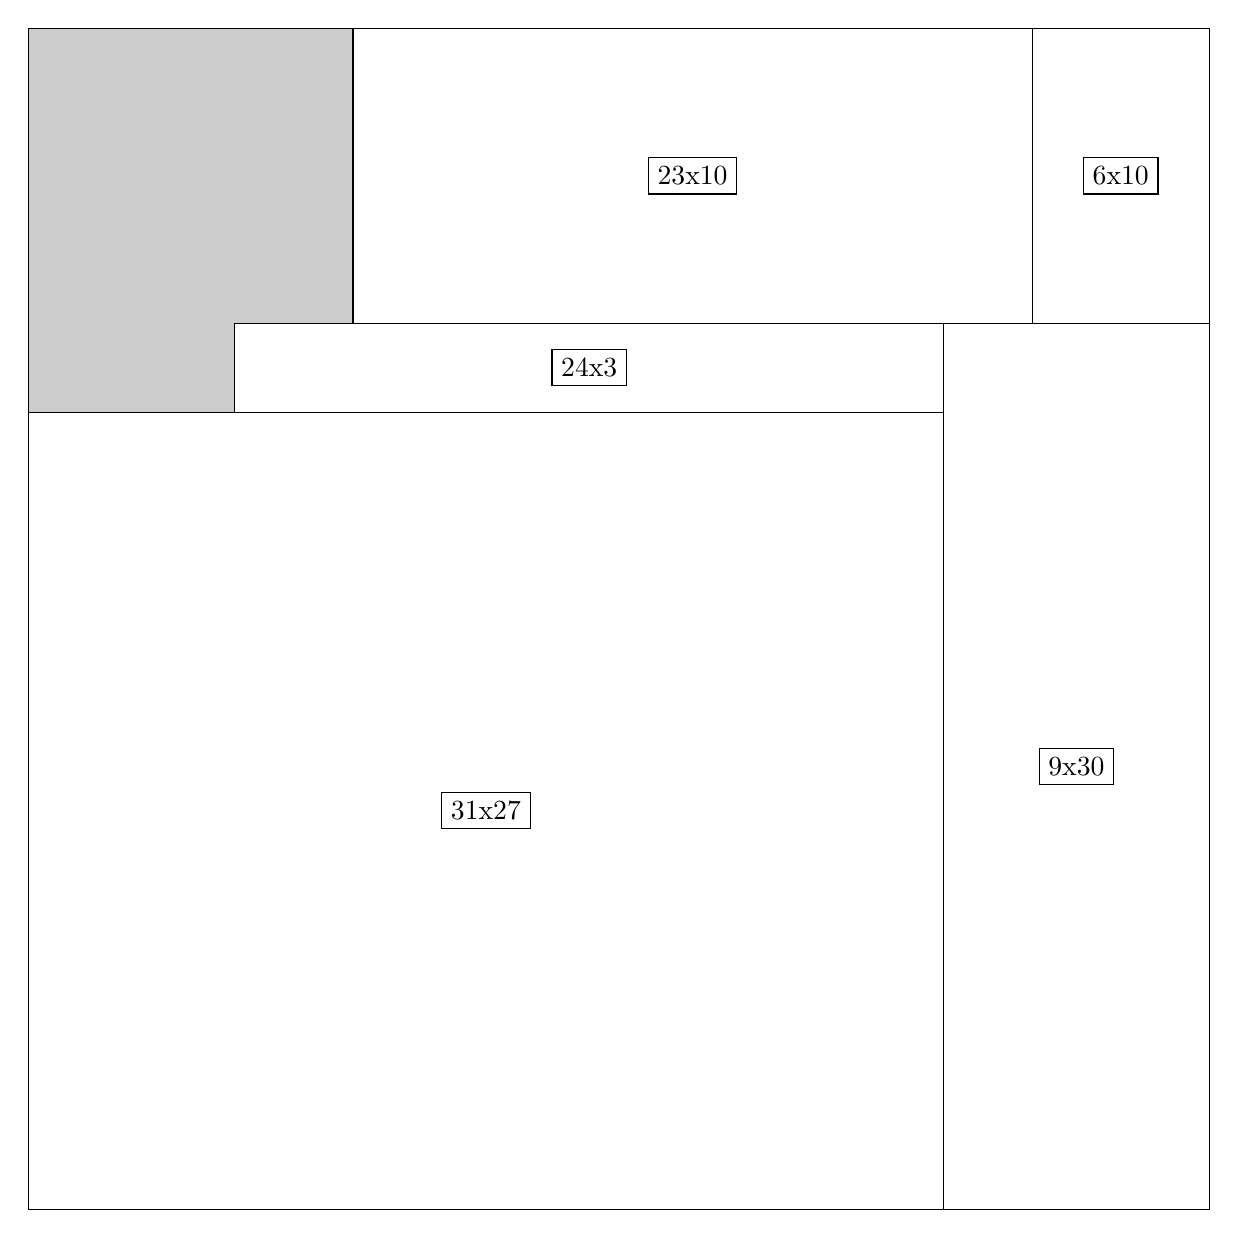
\begin{tikzpicture}[shorten >=1pt,scale=1.0,every node/.style={scale=1.0},->]
\tikzstyle{vertex}=[circle,fill=black!25,minimum size=14pt,inner sep=0pt]
\filldraw[fill=gray!40!white, draw=black] (0,0) rectangle (15.0,15.0);
\foreach \name/\x/\y/\w/\h in {31x27/0.0/0.0/11.625/10.125,9x30/11.625/0.0/3.375/11.25,23x10/4.125/11.25/8.625/3.75,24x3/2.625/10.125/9.0/1.125,6x10/12.75/11.25/2.25/3.75}
\filldraw[fill=white!40!white, draw=black] (\x,\y) rectangle node[draw] (\name) {\name} ++(\w,\h);
\end{tikzpicture}


w =31 , h =27 , x =0 , y =0 , v =837
\par
w =9 , h =30 , x =31 , y =0 , v =270
\par
w =23 , h =10 , x =11 , y =30 , v =230
\par
w =24 , h =3 , x =7 , y =27 , v =72
\par
w =6 , h =10 , x =34 , y =30 , v =60
\par
\newpage


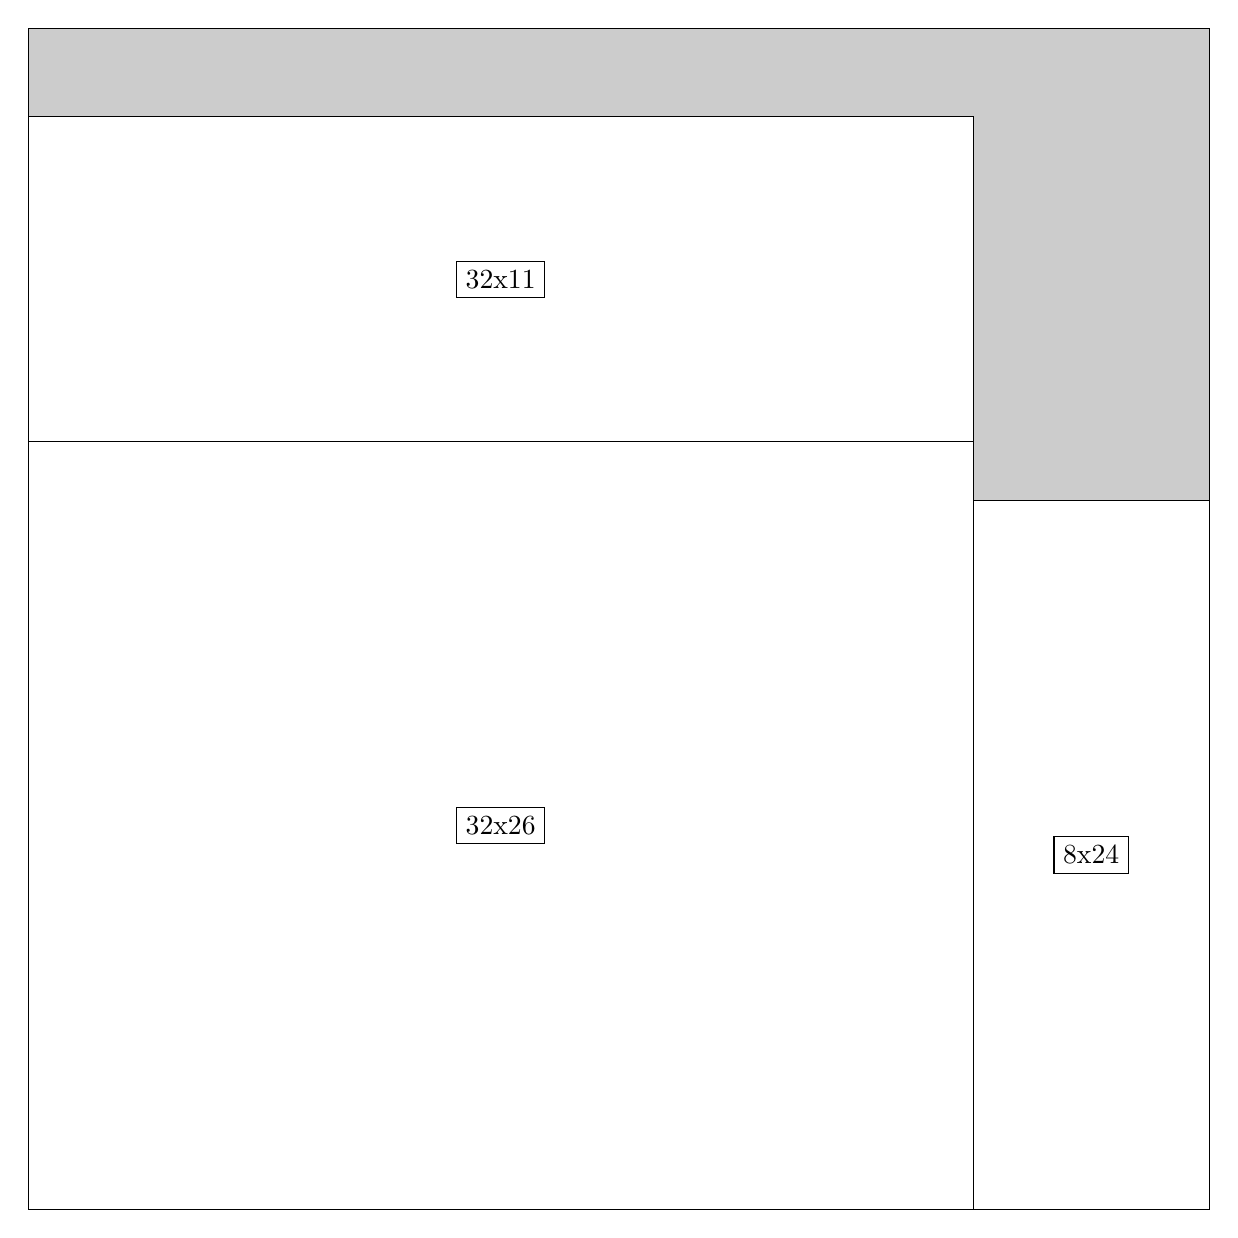
\begin{tikzpicture}[shorten >=1pt,scale=1.0,every node/.style={scale=1.0},->]
\tikzstyle{vertex}=[circle,fill=black!25,minimum size=14pt,inner sep=0pt]
\filldraw[fill=gray!40!white, draw=black] (0,0) rectangle (15.0,15.0);
\foreach \name/\x/\y/\w/\h in {32x26/0.0/0.0/12.0/9.75,32x11/0.0/9.75/12.0/4.125,8x24/12.0/0.0/3.0/9.0}
\filldraw[fill=white!40!white, draw=black] (\x,\y) rectangle node[draw] (\name) {\name} ++(\w,\h);
\end{tikzpicture}


w =32 , h =26 , x =0 , y =0 , v =832
\par
w =32 , h =11 , x =0 , y =26 , v =352
\par
w =8 , h =24 , x =32 , y =0 , v =192
\par
\newpage


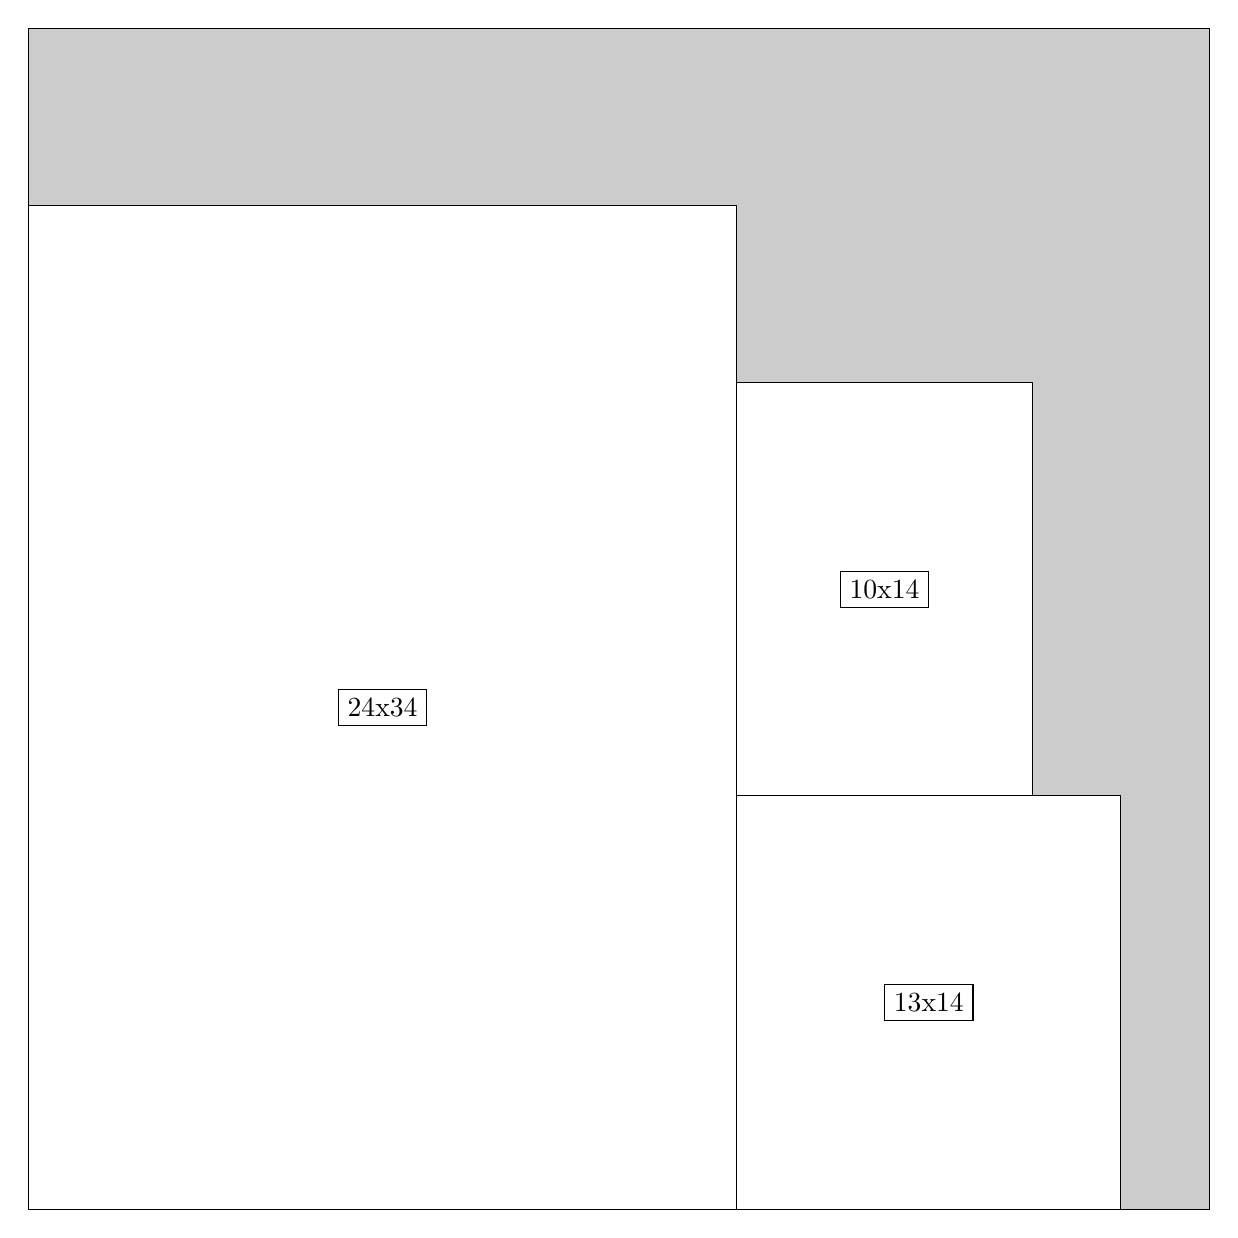
\begin{tikzpicture}[shorten >=1pt,scale=1.0,every node/.style={scale=1.0},->]
\tikzstyle{vertex}=[circle,fill=black!25,minimum size=14pt,inner sep=0pt]
\filldraw[fill=gray!40!white, draw=black] (0,0) rectangle (15.0,15.0);
\foreach \name/\x/\y/\w/\h in {24x34/0.0/0.0/9.0/12.75,13x14/9.0/0.0/4.875/5.25,10x14/9.0/5.25/3.75/5.25}
\filldraw[fill=white!40!white, draw=black] (\x,\y) rectangle node[draw] (\name) {\name} ++(\w,\h);
\end{tikzpicture}


w =24 , h =34 , x =0 , y =0 , v =816
\par
w =13 , h =14 , x =24 , y =0 , v =182
\par
w =10 , h =14 , x =24 , y =14 , v =140
\par
\newpage


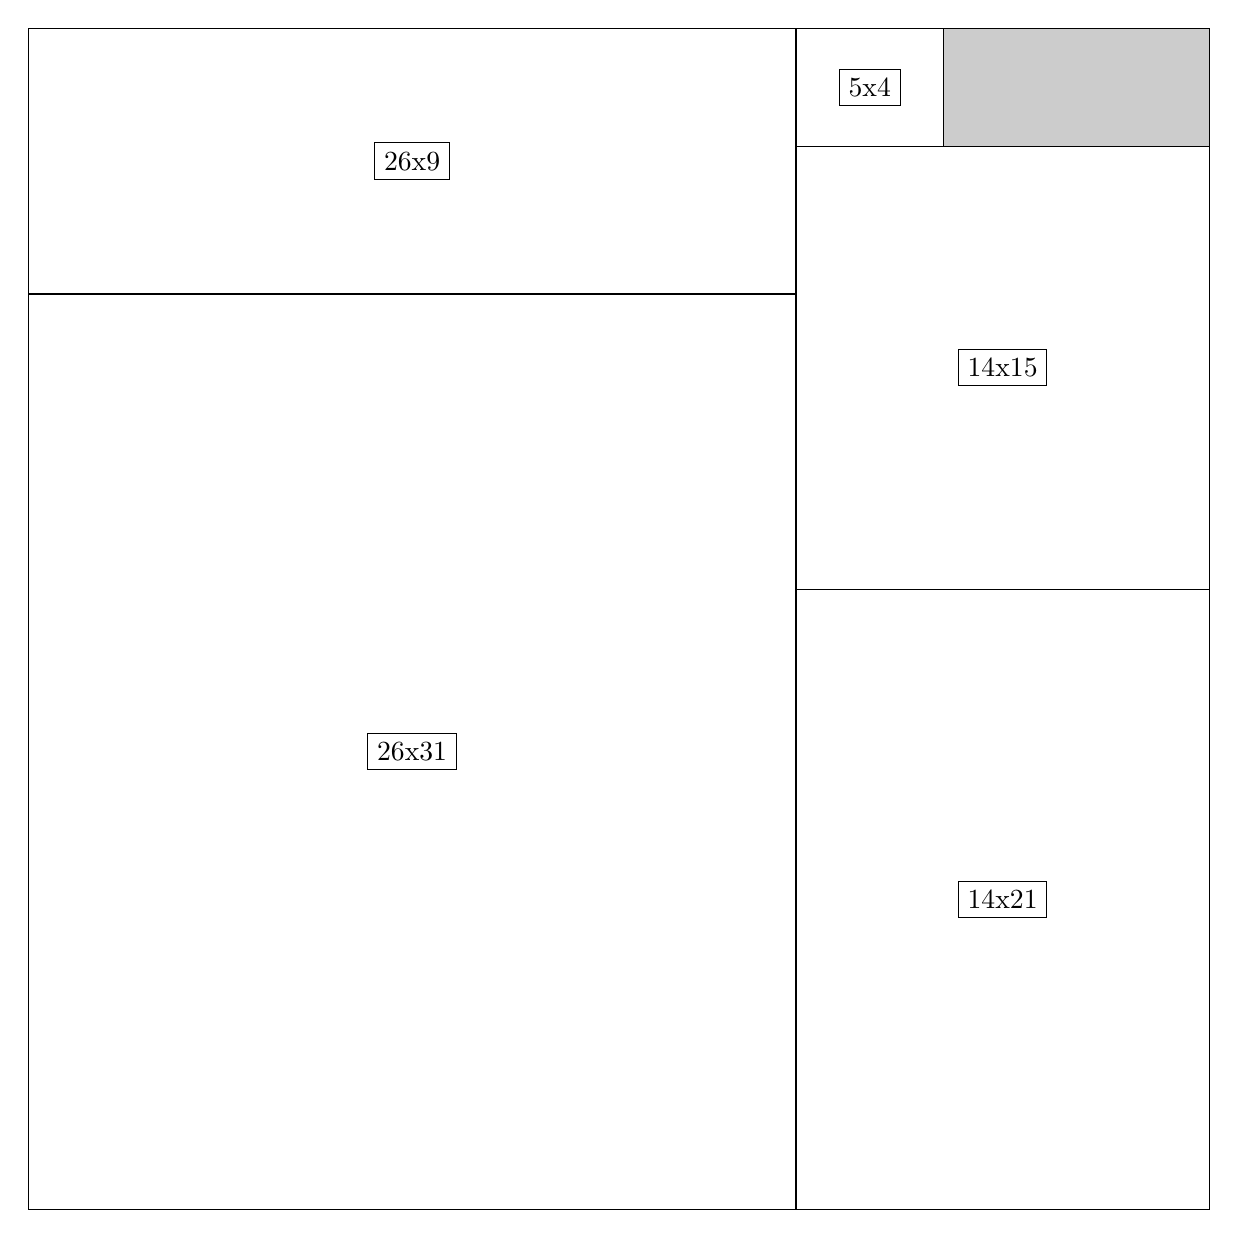
\begin{tikzpicture}[shorten >=1pt,scale=1.0,every node/.style={scale=1.0},->]
\tikzstyle{vertex}=[circle,fill=black!25,minimum size=14pt,inner sep=0pt]
\filldraw[fill=gray!40!white, draw=black] (0,0) rectangle (15.0,15.0);
\foreach \name/\x/\y/\w/\h in {14x21/9.75/0.0/5.25/7.875,26x31/0.0/0.0/9.75/11.625,26x9/0.0/11.625/9.75/3.375,14x15/9.75/7.875/5.25/5.625,5x4/9.75/13.5/1.875/1.5}
\filldraw[fill=white!40!white, draw=black] (\x,\y) rectangle node[draw] (\name) {\name} ++(\w,\h);
\end{tikzpicture}


w =14 , h =21 , x =26 , y =0 , v =294
\par
w =26 , h =31 , x =0 , y =0 , v =806
\par
w =26 , h =9 , x =0 , y =31 , v =234
\par
w =14 , h =15 , x =26 , y =21 , v =210
\par
w =5 , h =4 , x =26 , y =36 , v =20
\par
\newpage


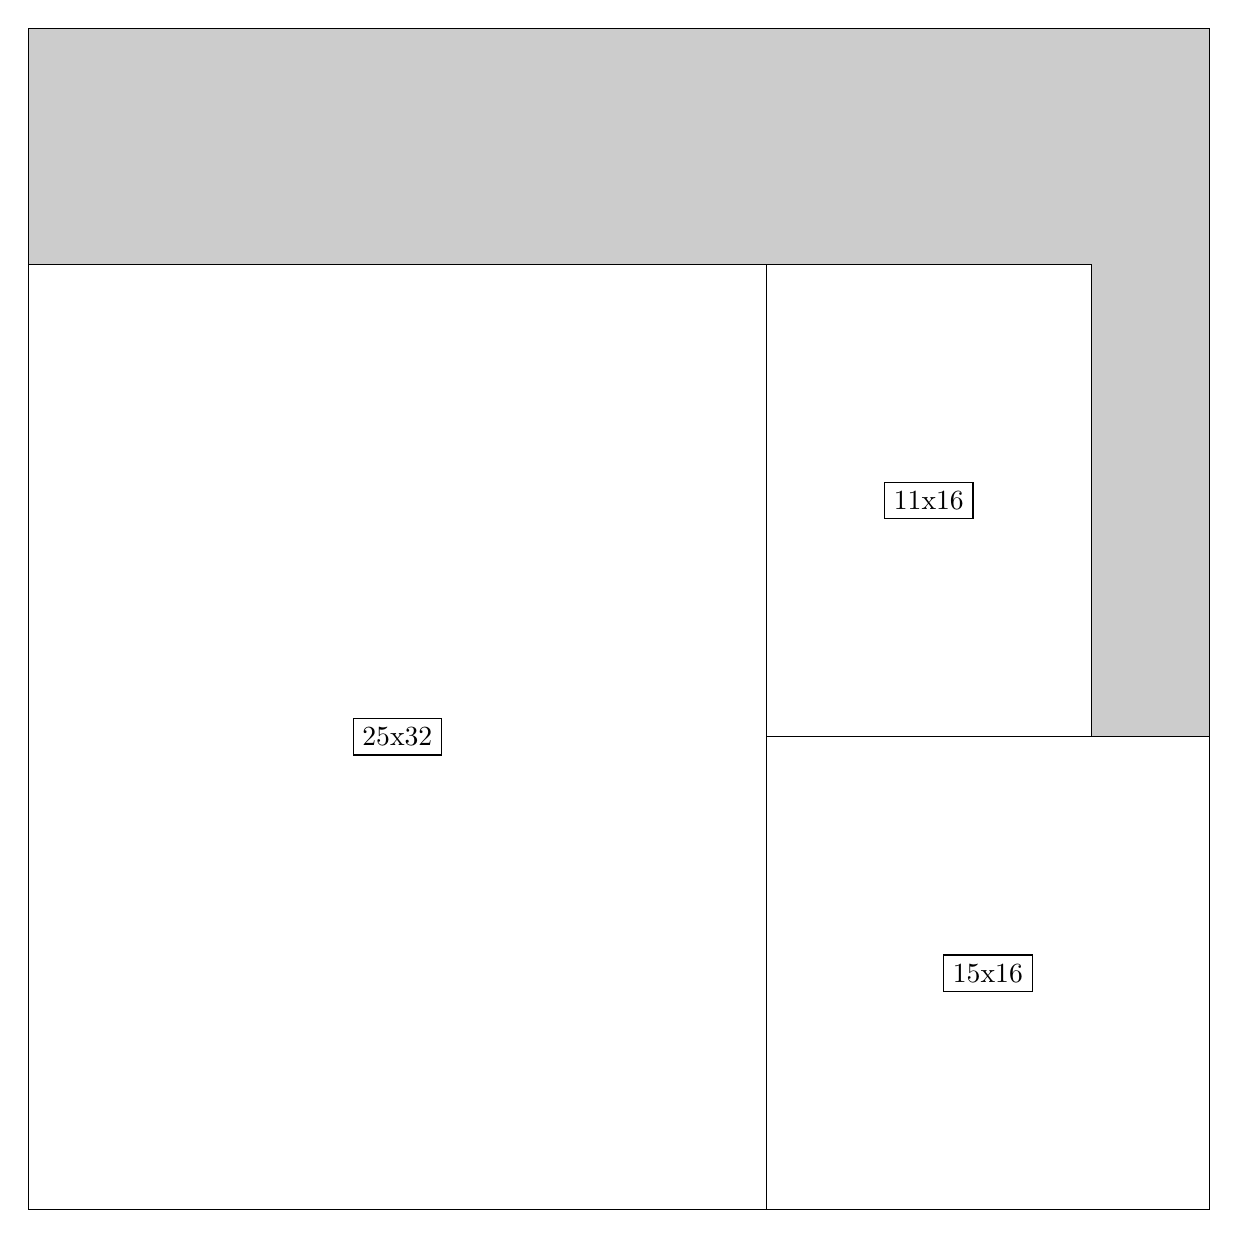
\begin{tikzpicture}[shorten >=1pt,scale=1.0,every node/.style={scale=1.0},->]
\tikzstyle{vertex}=[circle,fill=black!25,minimum size=14pt,inner sep=0pt]
\filldraw[fill=gray!40!white, draw=black] (0,0) rectangle (15.0,15.0);
\foreach \name/\x/\y/\w/\h in {25x32/0.0/0.0/9.375/12.0,15x16/9.375/0.0/5.625/6.0,11x16/9.375/6.0/4.125/6.0}
\filldraw[fill=white!40!white, draw=black] (\x,\y) rectangle node[draw] (\name) {\name} ++(\w,\h);
\end{tikzpicture}


w =25 , h =32 , x =0 , y =0 , v =800
\par
w =15 , h =16 , x =25 , y =0 , v =240
\par
w =11 , h =16 , x =25 , y =16 , v =176
\par
\newpage


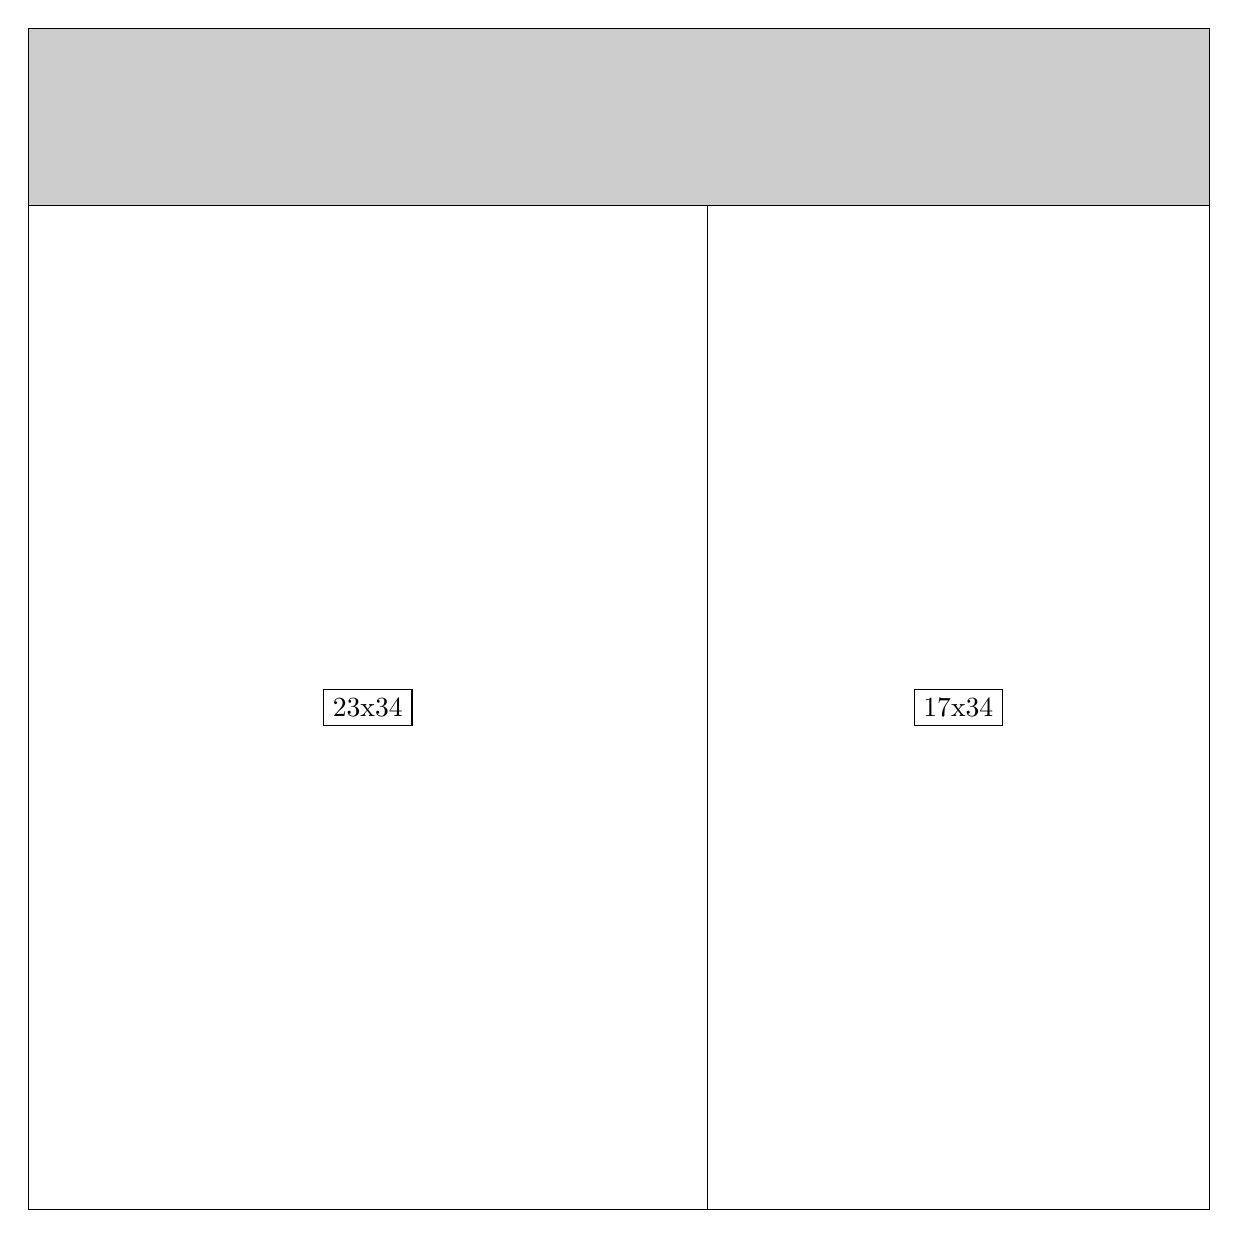
\begin{tikzpicture}[shorten >=1pt,scale=1.0,every node/.style={scale=1.0},->]
\tikzstyle{vertex}=[circle,fill=black!25,minimum size=14pt,inner sep=0pt]
\filldraw[fill=gray!40!white, draw=black] (0,0) rectangle (15.0,15.0);
\foreach \name/\x/\y/\w/\h in {23x34/0.0/0.0/8.625/12.75,17x34/8.625/0.0/6.375/12.75}
\filldraw[fill=white!40!white, draw=black] (\x,\y) rectangle node[draw] (\name) {\name} ++(\w,\h);
\end{tikzpicture}


w =23 , h =34 , x =0 , y =0 , v =782
\par
w =17 , h =34 , x =23 , y =0 , v =578
\par
\newpage


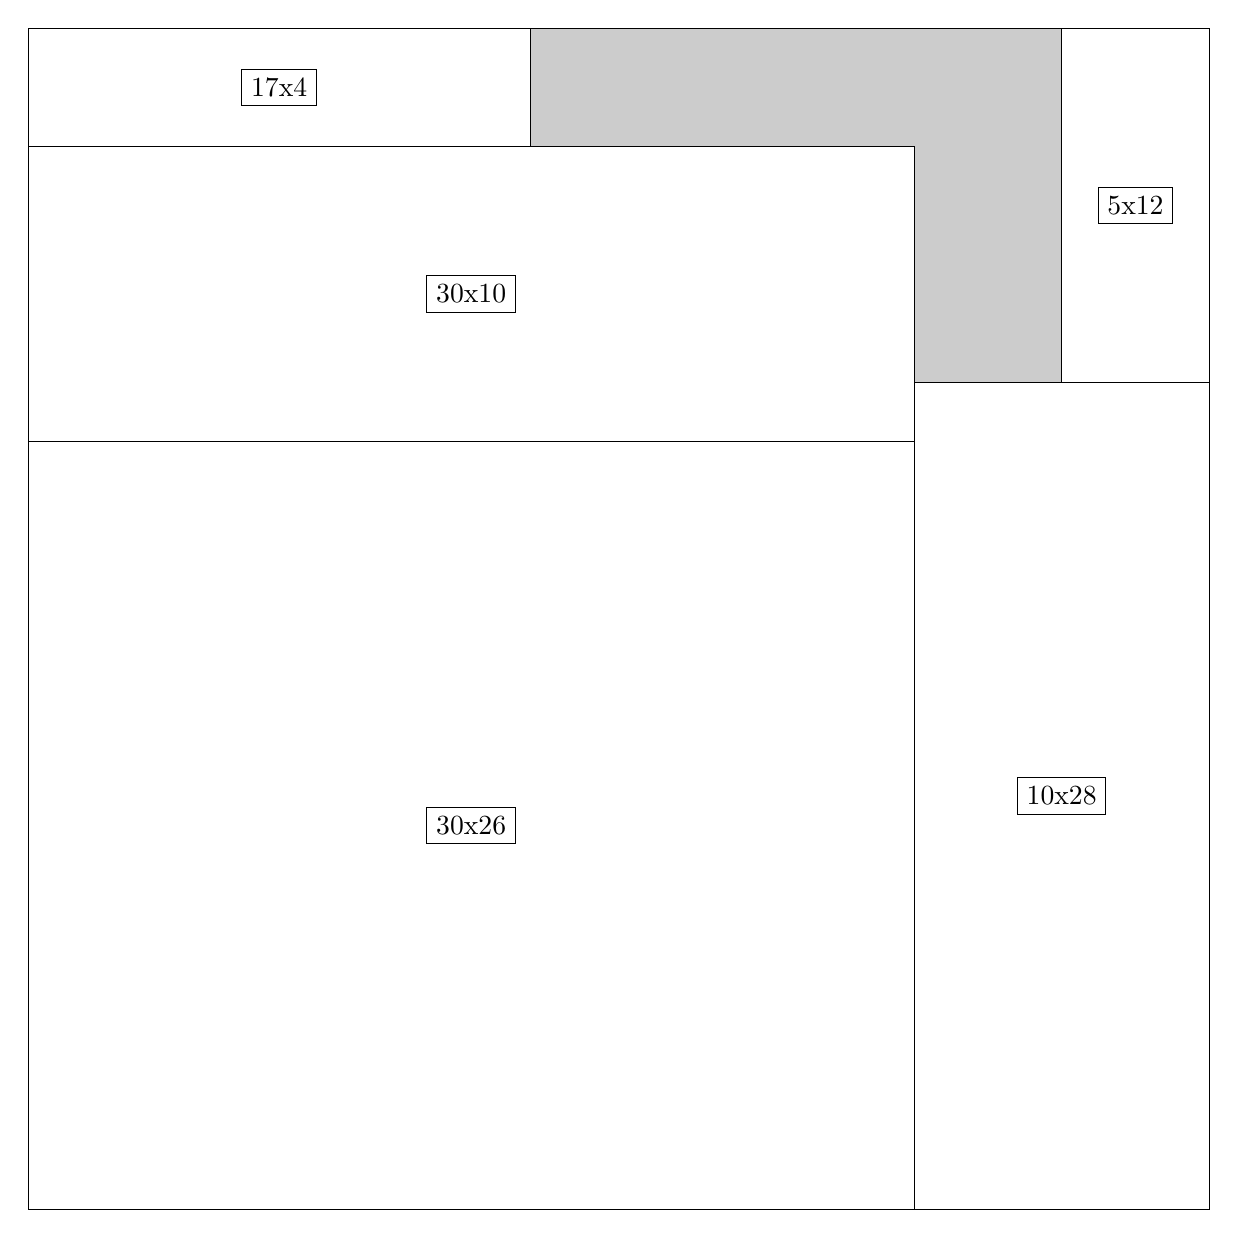
\begin{tikzpicture}[shorten >=1pt,scale=1.0,every node/.style={scale=1.0},->]
\tikzstyle{vertex}=[circle,fill=black!25,minimum size=14pt,inner sep=0pt]
\filldraw[fill=gray!40!white, draw=black] (0,0) rectangle (15.0,15.0);
\foreach \name/\x/\y/\w/\h in {30x26/0.0/0.0/11.25/9.75,30x10/0.0/9.75/11.25/3.75,10x28/11.25/0.0/3.75/10.5,17x4/0.0/13.5/6.375/1.5,5x12/13.125/10.5/1.875/4.5}
\filldraw[fill=white!40!white, draw=black] (\x,\y) rectangle node[draw] (\name) {\name} ++(\w,\h);
\end{tikzpicture}


w =30 , h =26 , x =0 , y =0 , v =780
\par
w =30 , h =10 , x =0 , y =26 , v =300
\par
w =10 , h =28 , x =30 , y =0 , v =280
\par
w =17 , h =4 , x =0 , y =36 , v =68
\par
w =5 , h =12 , x =35 , y =28 , v =60
\par
\newpage


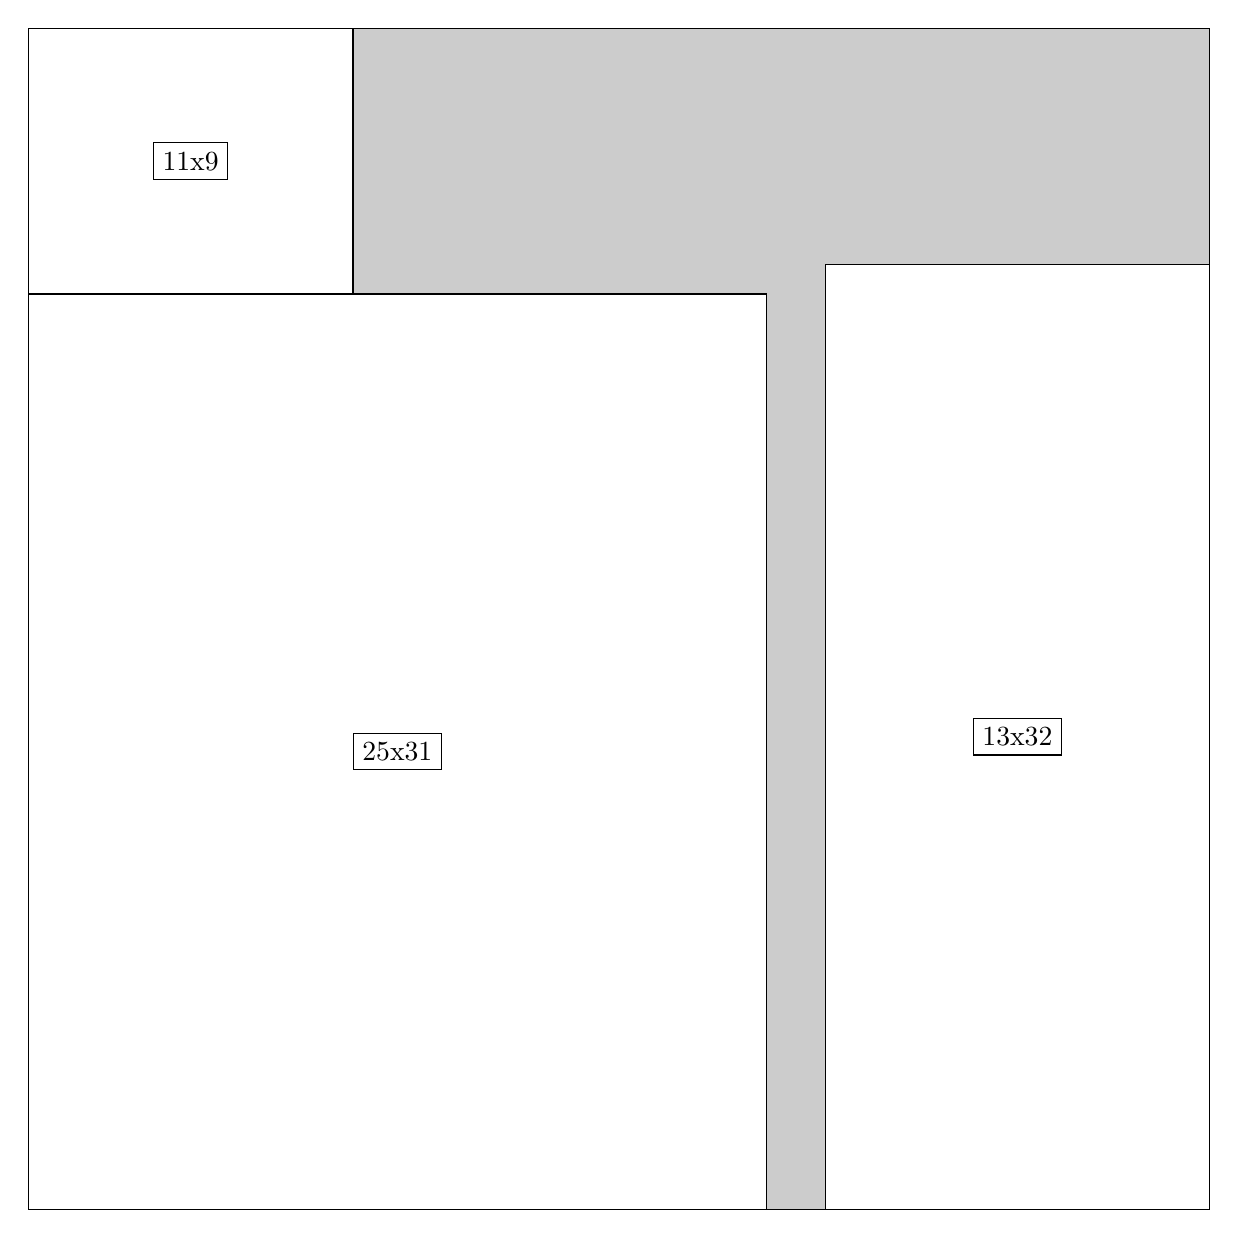
\begin{tikzpicture}[shorten >=1pt,scale=1.0,every node/.style={scale=1.0},->]
\tikzstyle{vertex}=[circle,fill=black!25,minimum size=14pt,inner sep=0pt]
\filldraw[fill=gray!40!white, draw=black] (0,0) rectangle (15.0,15.0);
\foreach \name/\x/\y/\w/\h in {25x31/0.0/0.0/9.375/11.625,13x32/10.125/0.0/4.875/12.0,11x9/0.0/11.625/4.125/3.375}
\filldraw[fill=white!40!white, draw=black] (\x,\y) rectangle node[draw] (\name) {\name} ++(\w,\h);
\end{tikzpicture}


w =25 , h =31 , x =0 , y =0 , v =775
\par
w =13 , h =32 , x =27 , y =0 , v =416
\par
w =11 , h =9 , x =0 , y =31 , v =99
\par
\newpage


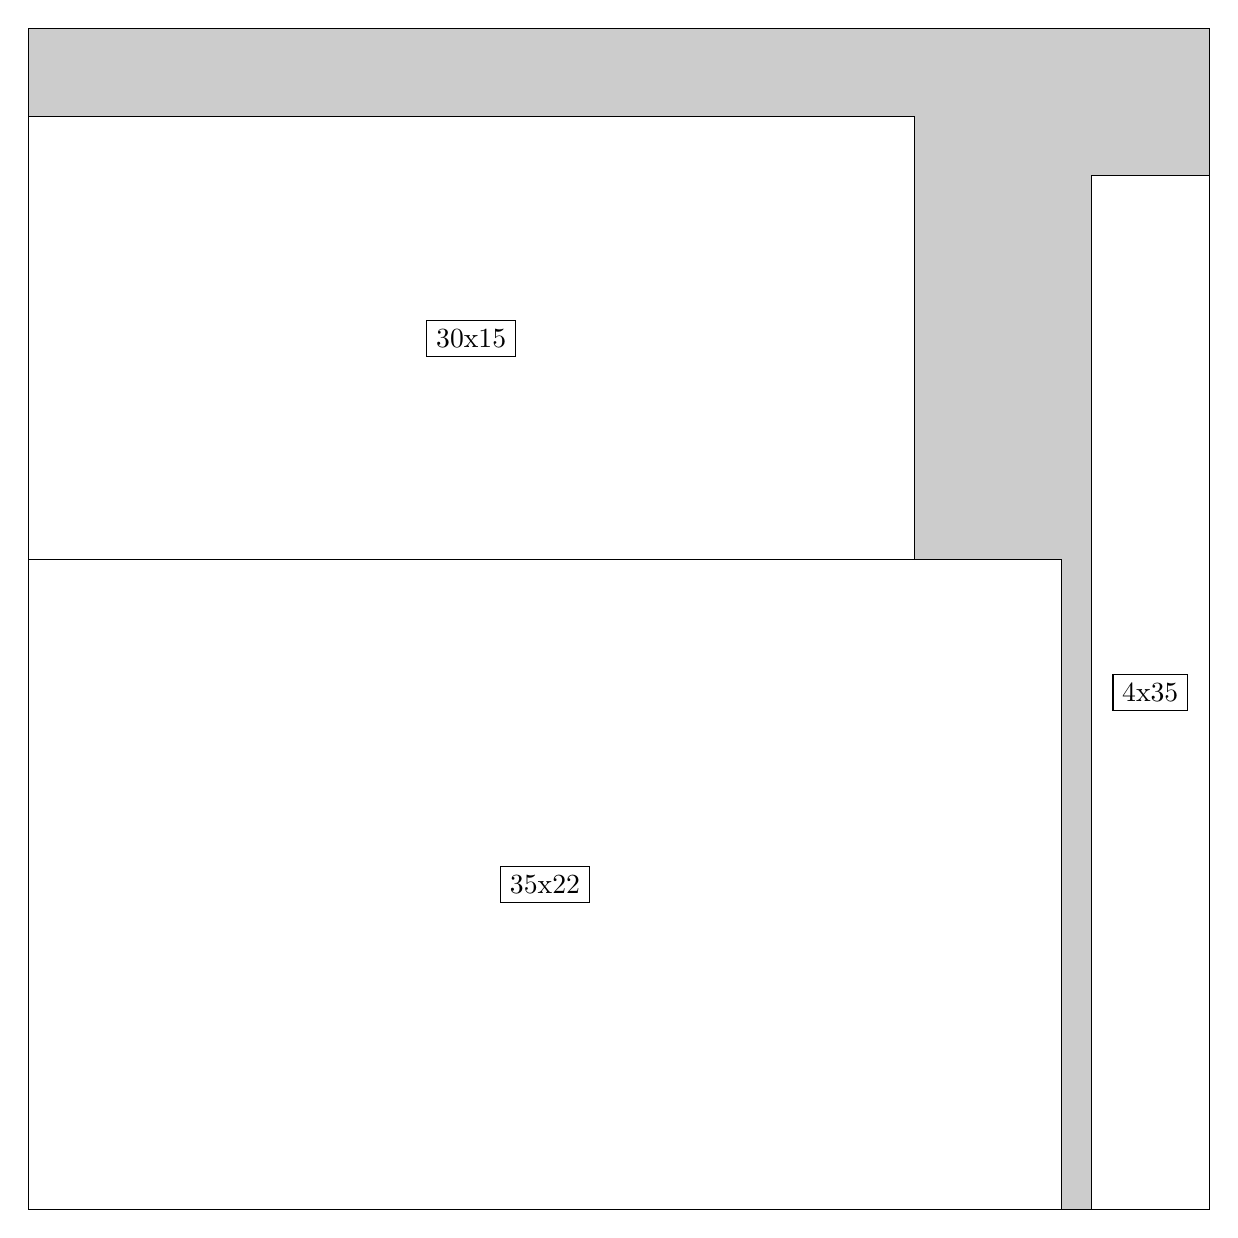
\begin{tikzpicture}[shorten >=1pt,scale=1.0,every node/.style={scale=1.0},->]
\tikzstyle{vertex}=[circle,fill=black!25,minimum size=14pt,inner sep=0pt]
\filldraw[fill=gray!40!white, draw=black] (0,0) rectangle (15.0,15.0);
\foreach \name/\x/\y/\w/\h in {35x22/0.0/0.0/13.125/8.25,30x15/0.0/8.25/11.25/5.625,4x35/13.5/0.0/1.5/13.125}
\filldraw[fill=white!40!white, draw=black] (\x,\y) rectangle node[draw] (\name) {\name} ++(\w,\h);
\end{tikzpicture}


w =35 , h =22 , x =0 , y =0 , v =770
\par
w =30 , h =15 , x =0 , y =22 , v =450
\par
w =4 , h =35 , x =36 , y =0 , v =140
\par
\newpage


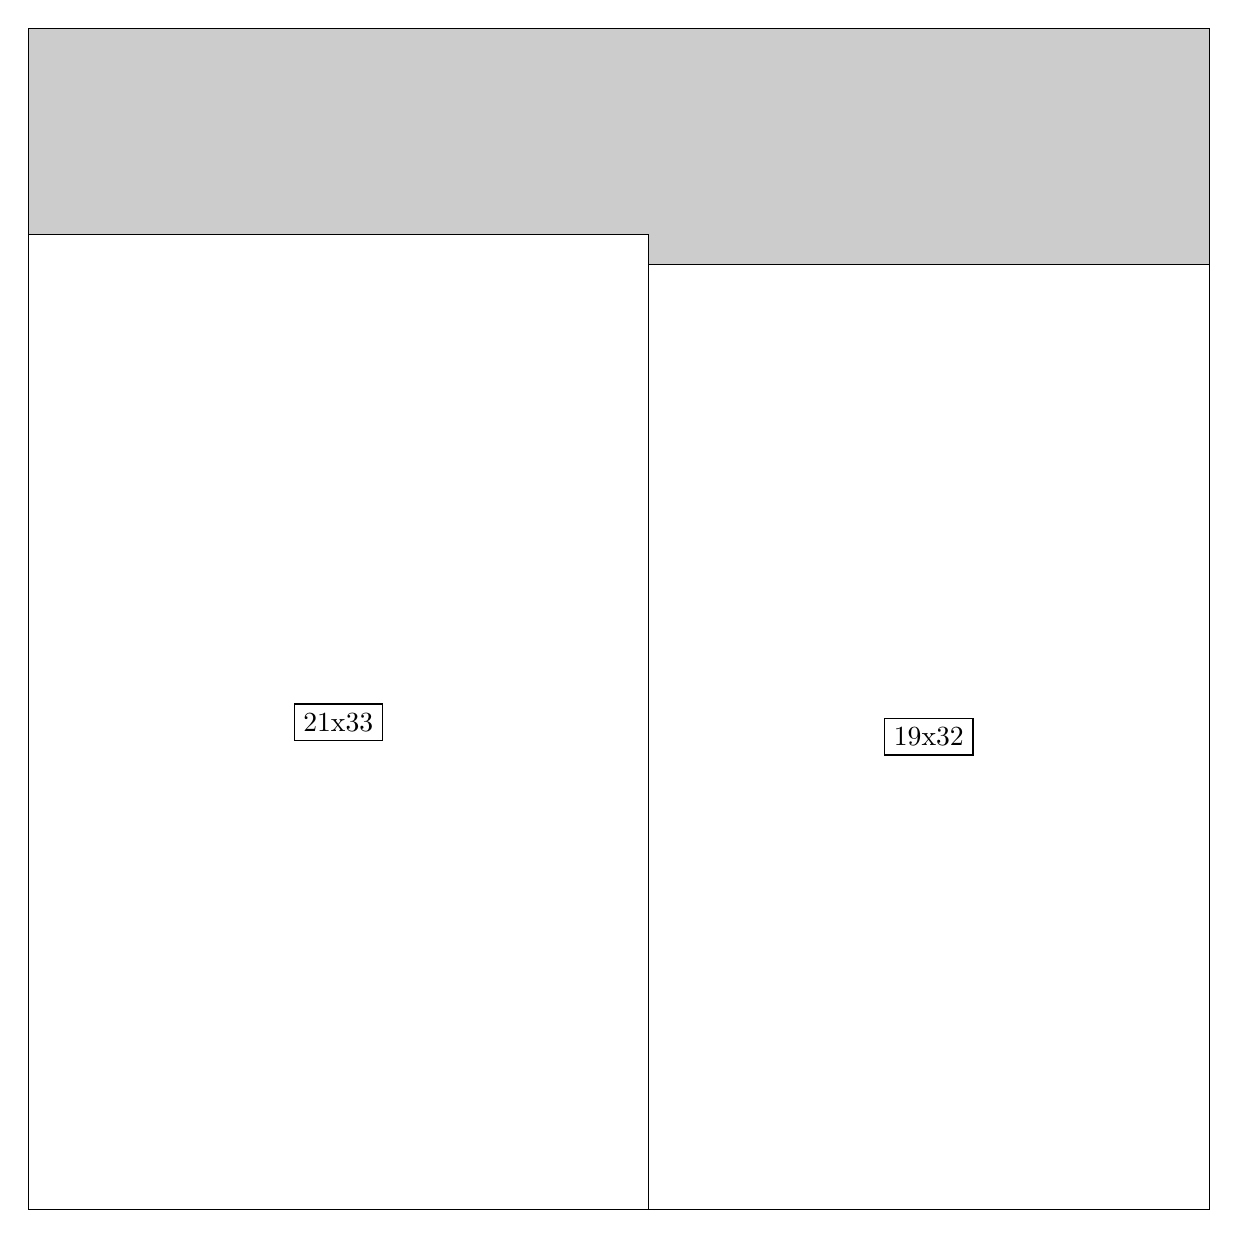
\begin{tikzpicture}[shorten >=1pt,scale=1.0,every node/.style={scale=1.0},->]
\tikzstyle{vertex}=[circle,fill=black!25,minimum size=14pt,inner sep=0pt]
\filldraw[fill=gray!40!white, draw=black] (0,0) rectangle (15.0,15.0);
\foreach \name/\x/\y/\w/\h in {21x33/0.0/0.0/7.875/12.375,19x32/7.875/0.0/7.125/12.0}
\filldraw[fill=white!40!white, draw=black] (\x,\y) rectangle node[draw] (\name) {\name} ++(\w,\h);
\end{tikzpicture}


w =21 , h =33 , x =0 , y =0 , v =693
\par
w =19 , h =32 , x =21 , y =0 , v =608
\par
\newpage


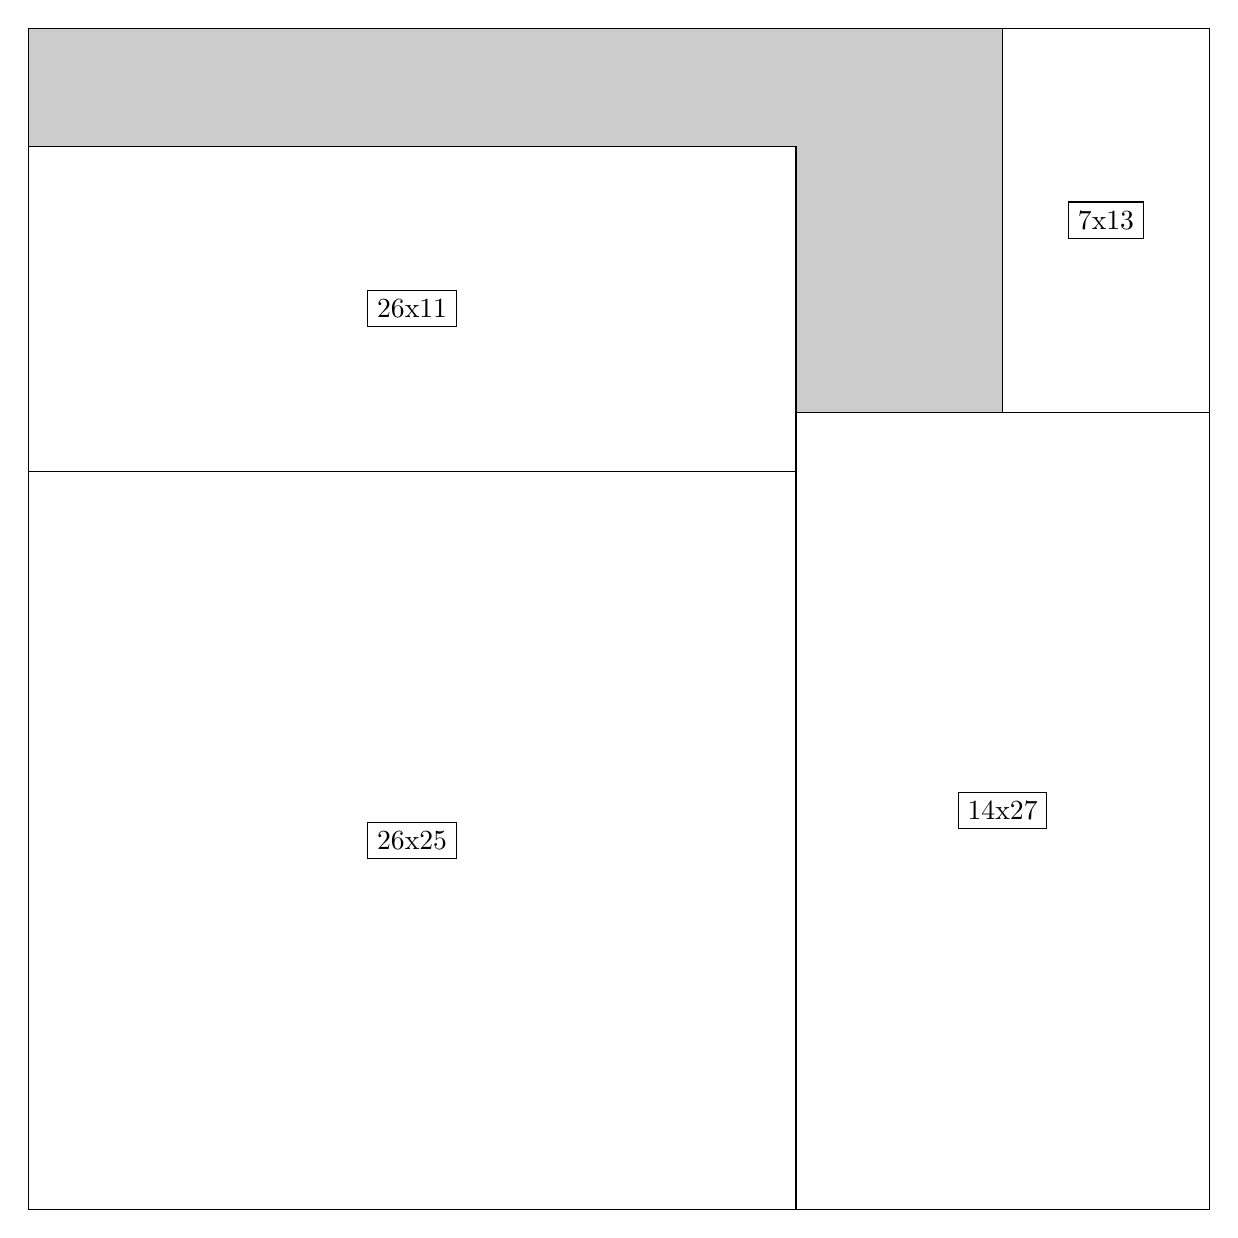
\begin{tikzpicture}[shorten >=1pt,scale=1.0,every node/.style={scale=1.0},->]
\tikzstyle{vertex}=[circle,fill=black!25,minimum size=14pt,inner sep=0pt]
\filldraw[fill=gray!40!white, draw=black] (0,0) rectangle (15.0,15.0);
\foreach \name/\x/\y/\w/\h in {26x25/0.0/0.0/9.75/9.375,14x27/9.75/0.0/5.25/10.125,26x11/0.0/9.375/9.75/4.125,7x13/12.375/10.125/2.625/4.875}
\filldraw[fill=white!40!white, draw=black] (\x,\y) rectangle node[draw] (\name) {\name} ++(\w,\h);
\end{tikzpicture}


w =26 , h =25 , x =0 , y =0 , v =650
\par
w =14 , h =27 , x =26 , y =0 , v =378
\par
w =26 , h =11 , x =0 , y =25 , v =286
\par
w =7 , h =13 , x =33 , y =27 , v =91
\par
\newpage


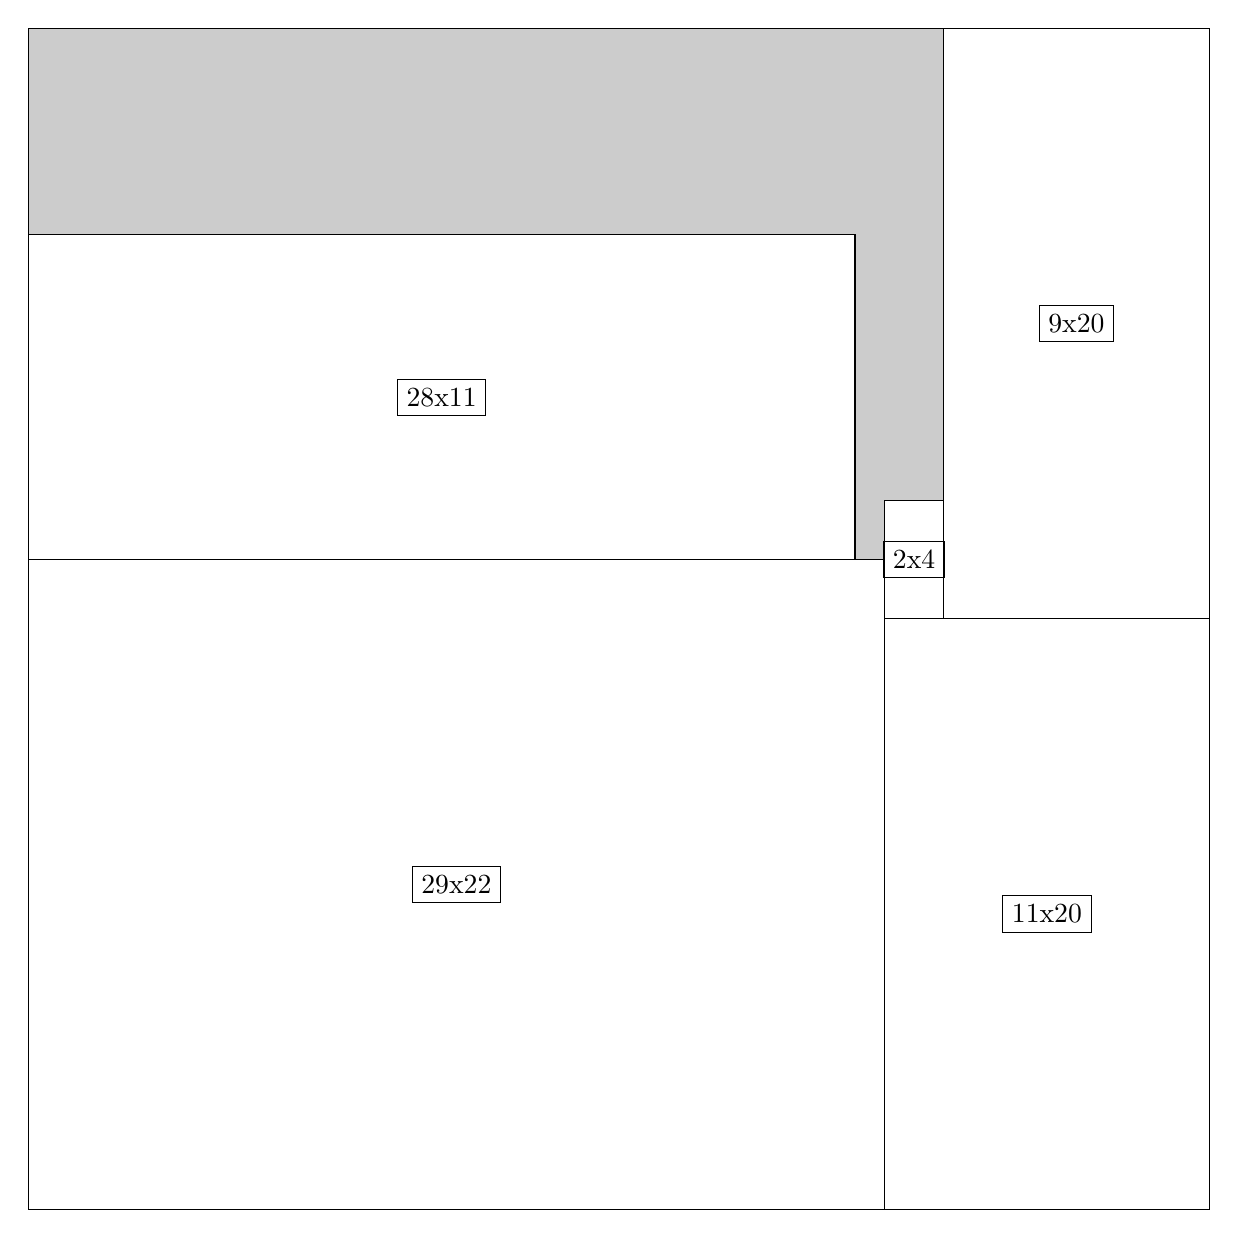
\begin{tikzpicture}[shorten >=1pt,scale=1.0,every node/.style={scale=1.0},->]
\tikzstyle{vertex}=[circle,fill=black!25,minimum size=14pt,inner sep=0pt]
\filldraw[fill=gray!40!white, draw=black] (0,0) rectangle (15.0,15.0);
\foreach \name/\x/\y/\w/\h in {29x22/0.0/0.0/10.875/8.25,28x11/0.0/8.25/10.5/4.125,11x20/10.875/0.0/4.125/7.5,9x20/11.625/7.5/3.375/7.5,2x4/10.875/7.5/0.75/1.5}
\filldraw[fill=white!40!white, draw=black] (\x,\y) rectangle node[draw] (\name) {\name} ++(\w,\h);
\end{tikzpicture}


w =29 , h =22 , x =0 , y =0 , v =638
\par
w =28 , h =11 , x =0 , y =22 , v =308
\par
w =11 , h =20 , x =29 , y =0 , v =220
\par
w =9 , h =20 , x =31 , y =20 , v =180
\par
w =2 , h =4 , x =29 , y =20 , v =8
\par
\newpage


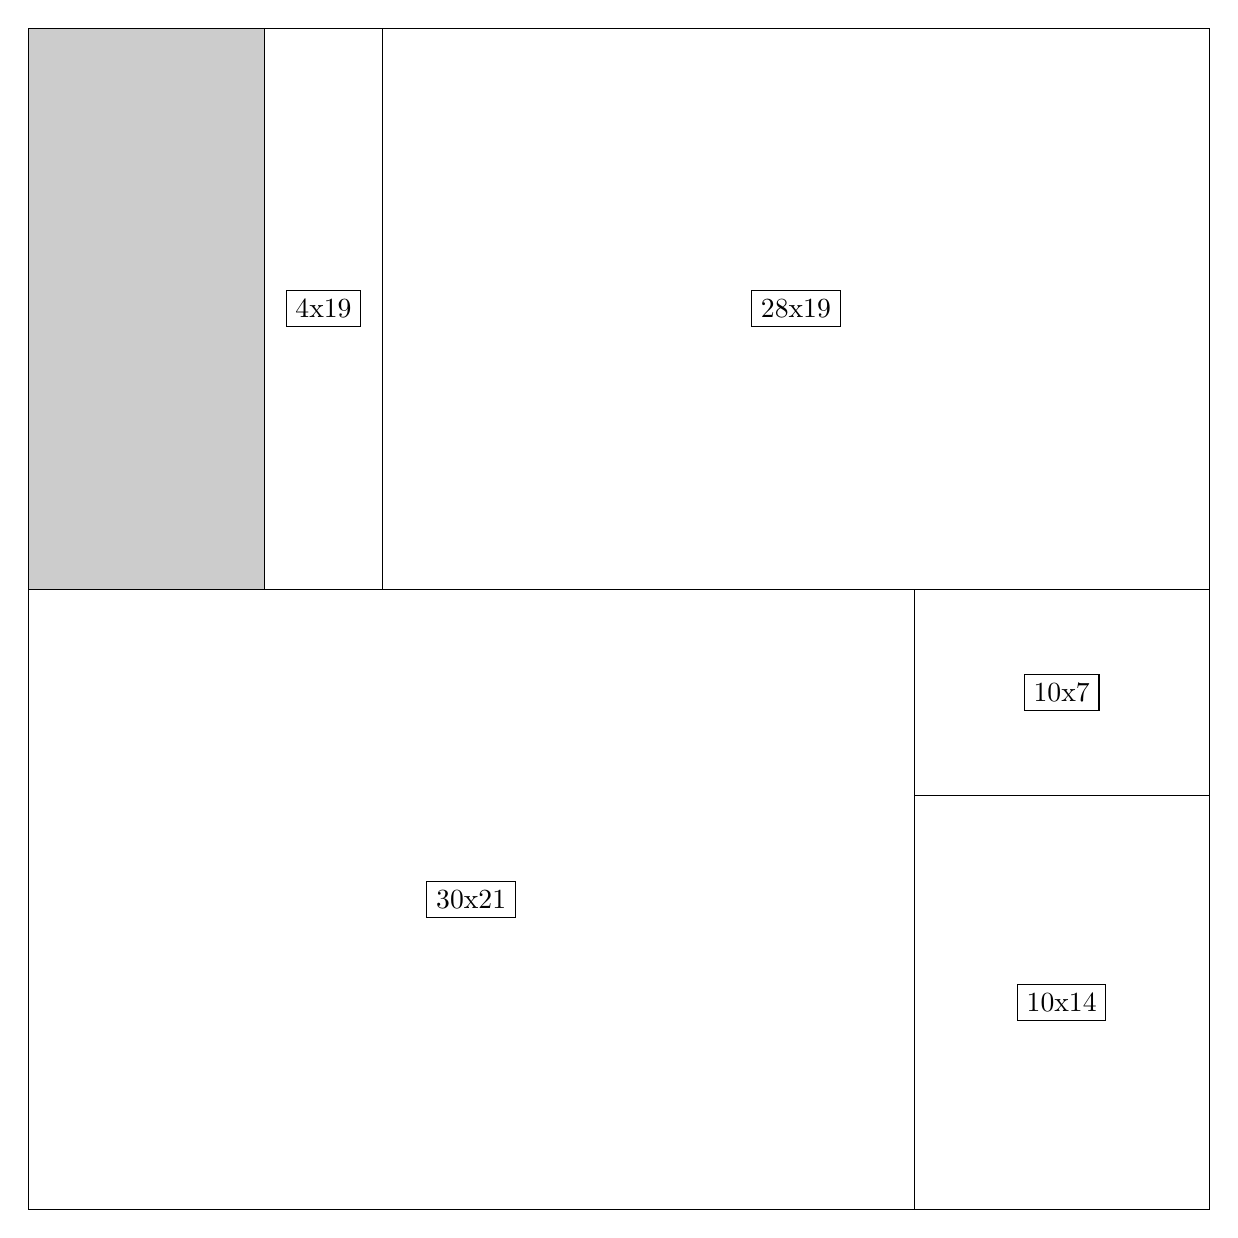
\begin{tikzpicture}[shorten >=1pt,scale=1.0,every node/.style={scale=1.0},->]
\tikzstyle{vertex}=[circle,fill=black!25,minimum size=14pt,inner sep=0pt]
\filldraw[fill=gray!40!white, draw=black] (0,0) rectangle (15.0,15.0);
\foreach \name/\x/\y/\w/\h in {30x21/0.0/0.0/11.25/7.875,28x19/4.5/7.875/10.5/7.125,10x14/11.25/0.0/3.75/5.25,4x19/3.0/7.875/1.5/7.125,10x7/11.25/5.25/3.75/2.625}
\filldraw[fill=white!40!white, draw=black] (\x,\y) rectangle node[draw] (\name) {\name} ++(\w,\h);
\end{tikzpicture}


w =30 , h =21 , x =0 , y =0 , v =630
\par
w =28 , h =19 , x =12 , y =21 , v =532
\par
w =10 , h =14 , x =30 , y =0 , v =140
\par
w =4 , h =19 , x =8 , y =21 , v =76
\par
w =10 , h =7 , x =30 , y =14 , v =70
\par
\newpage


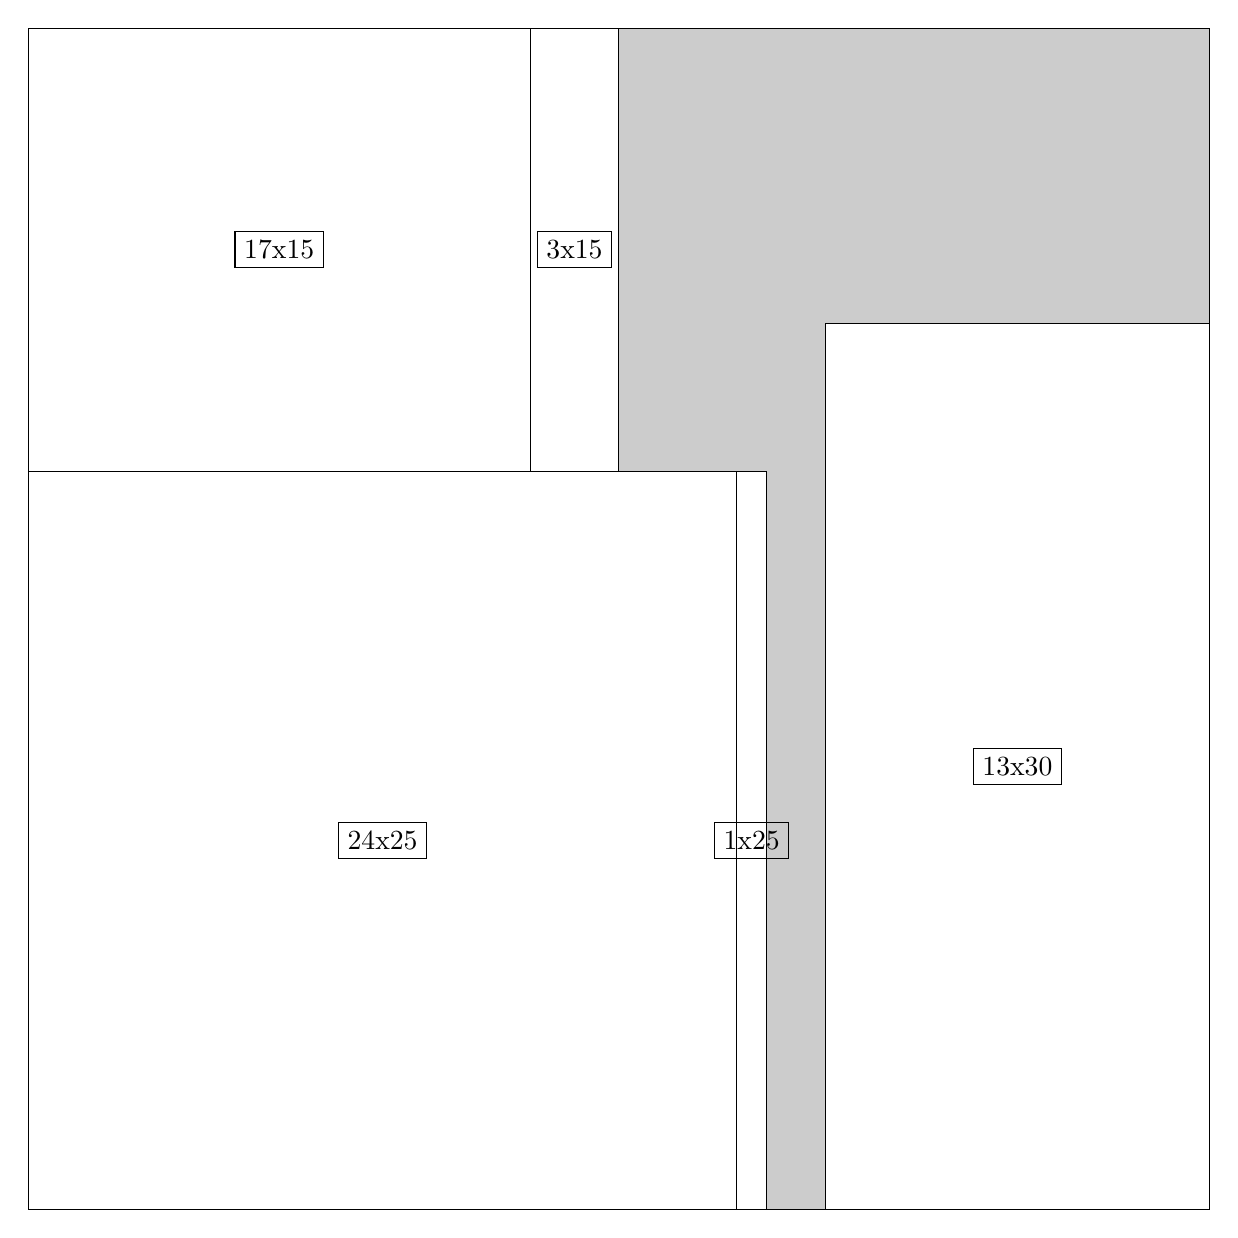
\begin{tikzpicture}[shorten >=1pt,scale=1.0,every node/.style={scale=1.0},->]
\tikzstyle{vertex}=[circle,fill=black!25,minimum size=14pt,inner sep=0pt]
\filldraw[fill=gray!40!white, draw=black] (0,0) rectangle (15.0,15.0);
\foreach \name/\x/\y/\w/\h in {24x25/0.0/0.0/9.0/9.375,13x30/10.125/0.0/4.875/11.25,17x15/0.0/9.375/6.375/5.625,3x15/6.375/9.375/1.125/5.625,1x25/9.0/0.0/0.375/9.375}
\filldraw[fill=white!40!white, draw=black] (\x,\y) rectangle node[draw] (\name) {\name} ++(\w,\h);
\end{tikzpicture}


w =24 , h =25 , x =0 , y =0 , v =600
\par
w =13 , h =30 , x =27 , y =0 , v =390
\par
w =17 , h =15 , x =0 , y =25 , v =255
\par
w =3 , h =15 , x =17 , y =25 , v =45
\par
w =1 , h =25 , x =24 , y =0 , v =25
\par
\newpage


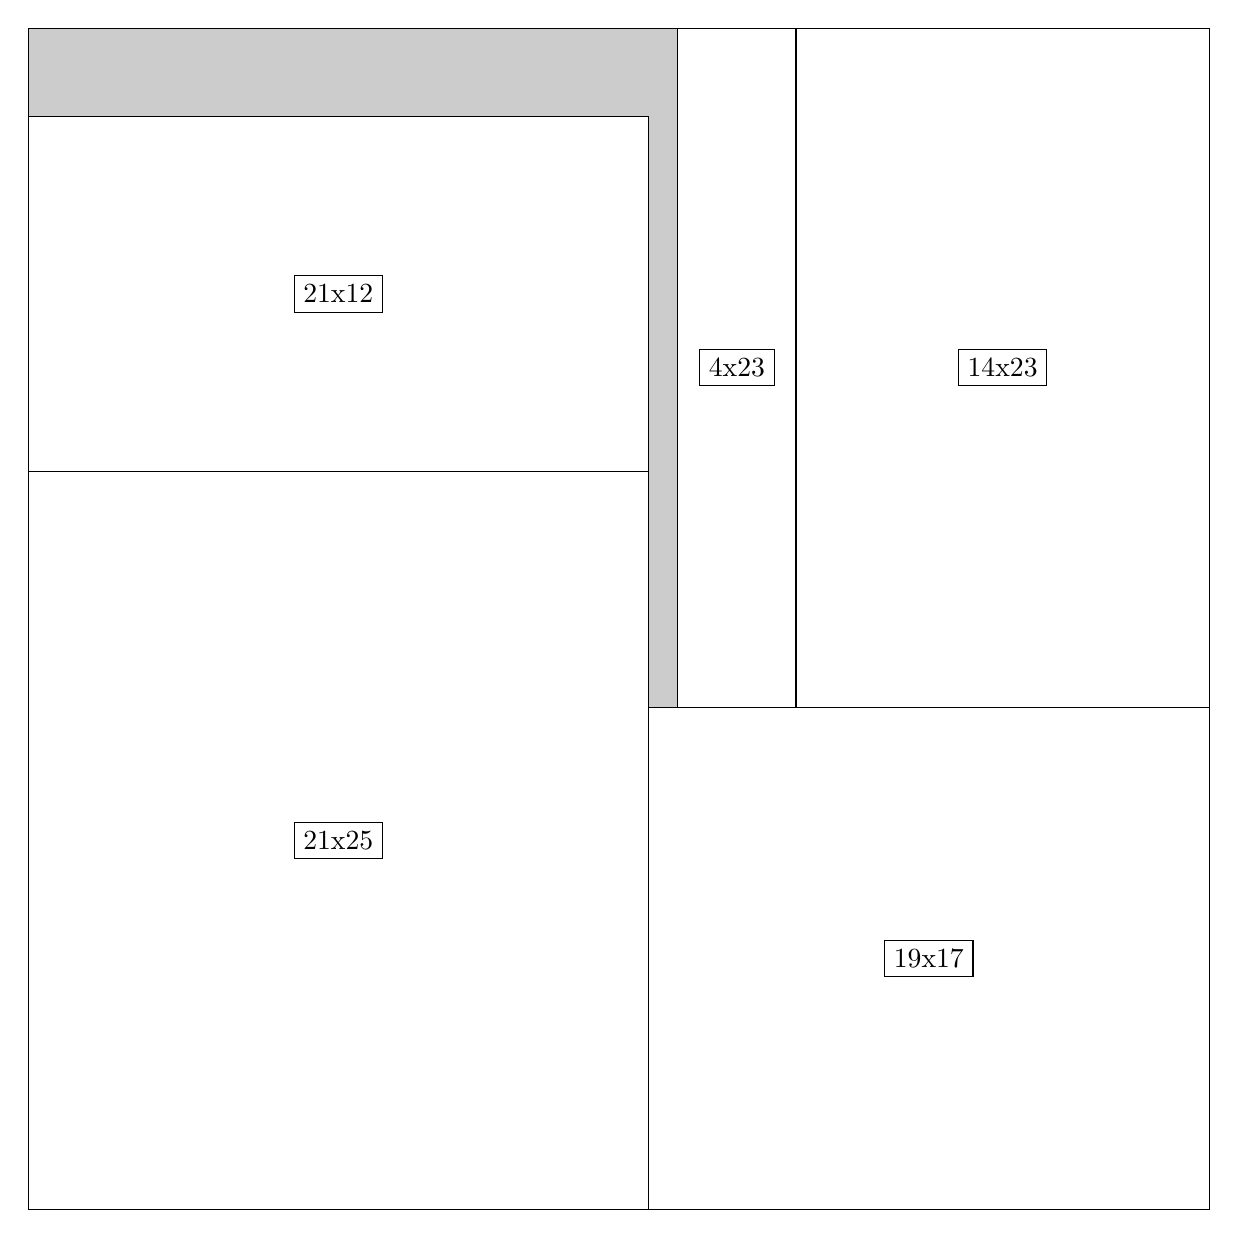
\begin{tikzpicture}[shorten >=1pt,scale=1.0,every node/.style={scale=1.0},->]
\tikzstyle{vertex}=[circle,fill=black!25,minimum size=14pt,inner sep=0pt]
\filldraw[fill=gray!40!white, draw=black] (0,0) rectangle (15.0,15.0);
\foreach \name/\x/\y/\w/\h in {21x25/0.0/0.0/7.875/9.375,19x17/7.875/0.0/7.125/6.375,14x23/9.75/6.375/5.25/8.625,21x12/0.0/9.375/7.875/4.5,4x23/8.25/6.375/1.5/8.625}
\filldraw[fill=white!40!white, draw=black] (\x,\y) rectangle node[draw] (\name) {\name} ++(\w,\h);
\end{tikzpicture}


w =21 , h =25 , x =0 , y =0 , v =525
\par
w =19 , h =17 , x =21 , y =0 , v =323
\par
w =14 , h =23 , x =26 , y =17 , v =322
\par
w =21 , h =12 , x =0 , y =25 , v =252
\par
w =4 , h =23 , x =22 , y =17 , v =92
\par
\newpage


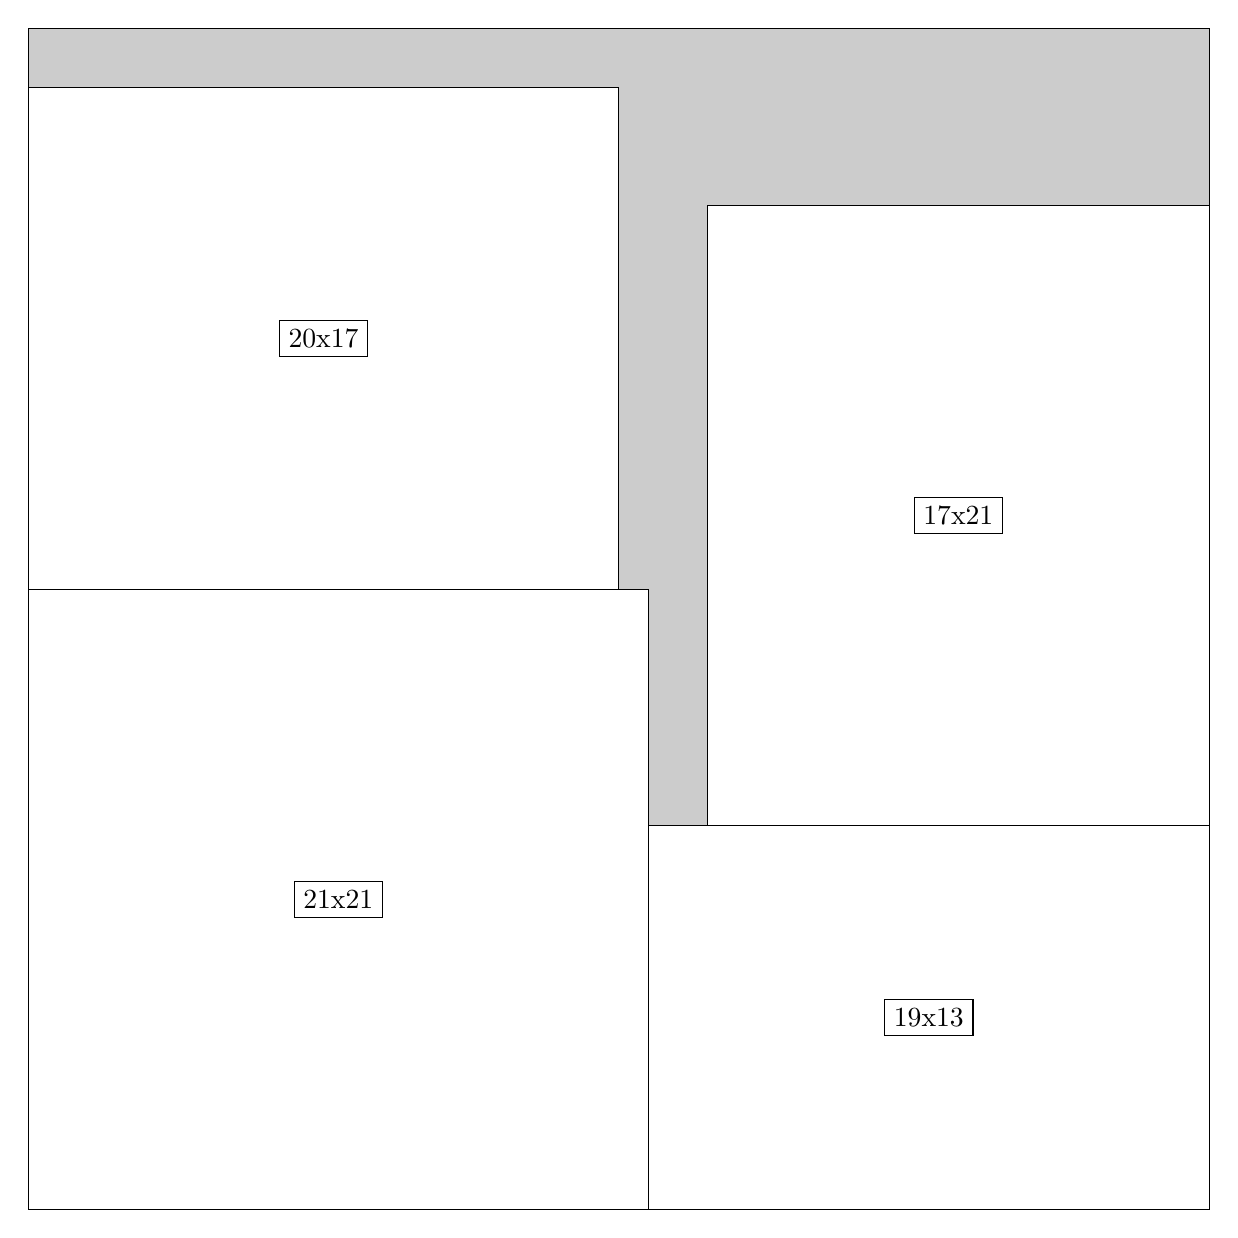
\begin{tikzpicture}[shorten >=1pt,scale=1.0,every node/.style={scale=1.0},->]
\tikzstyle{vertex}=[circle,fill=black!25,minimum size=14pt,inner sep=0pt]
\filldraw[fill=gray!40!white, draw=black] (0,0) rectangle (15.0,15.0);
\foreach \name/\x/\y/\w/\h in {21x21/0.0/0.0/7.875/7.875,17x21/8.625/4.875/6.375/7.875,20x17/0.0/7.875/7.5/6.375,19x13/7.875/0.0/7.125/4.875}
\filldraw[fill=white!40!white, draw=black] (\x,\y) rectangle node[draw] (\name) {\name} ++(\w,\h);
\end{tikzpicture}


w =21 , h =21 , x =0 , y =0 , v =441
\par
w =17 , h =21 , x =23 , y =13 , v =357
\par
w =20 , h =17 , x =0 , y =21 , v =340
\par
w =19 , h =13 , x =21 , y =0 , v =247
\par
\newpage


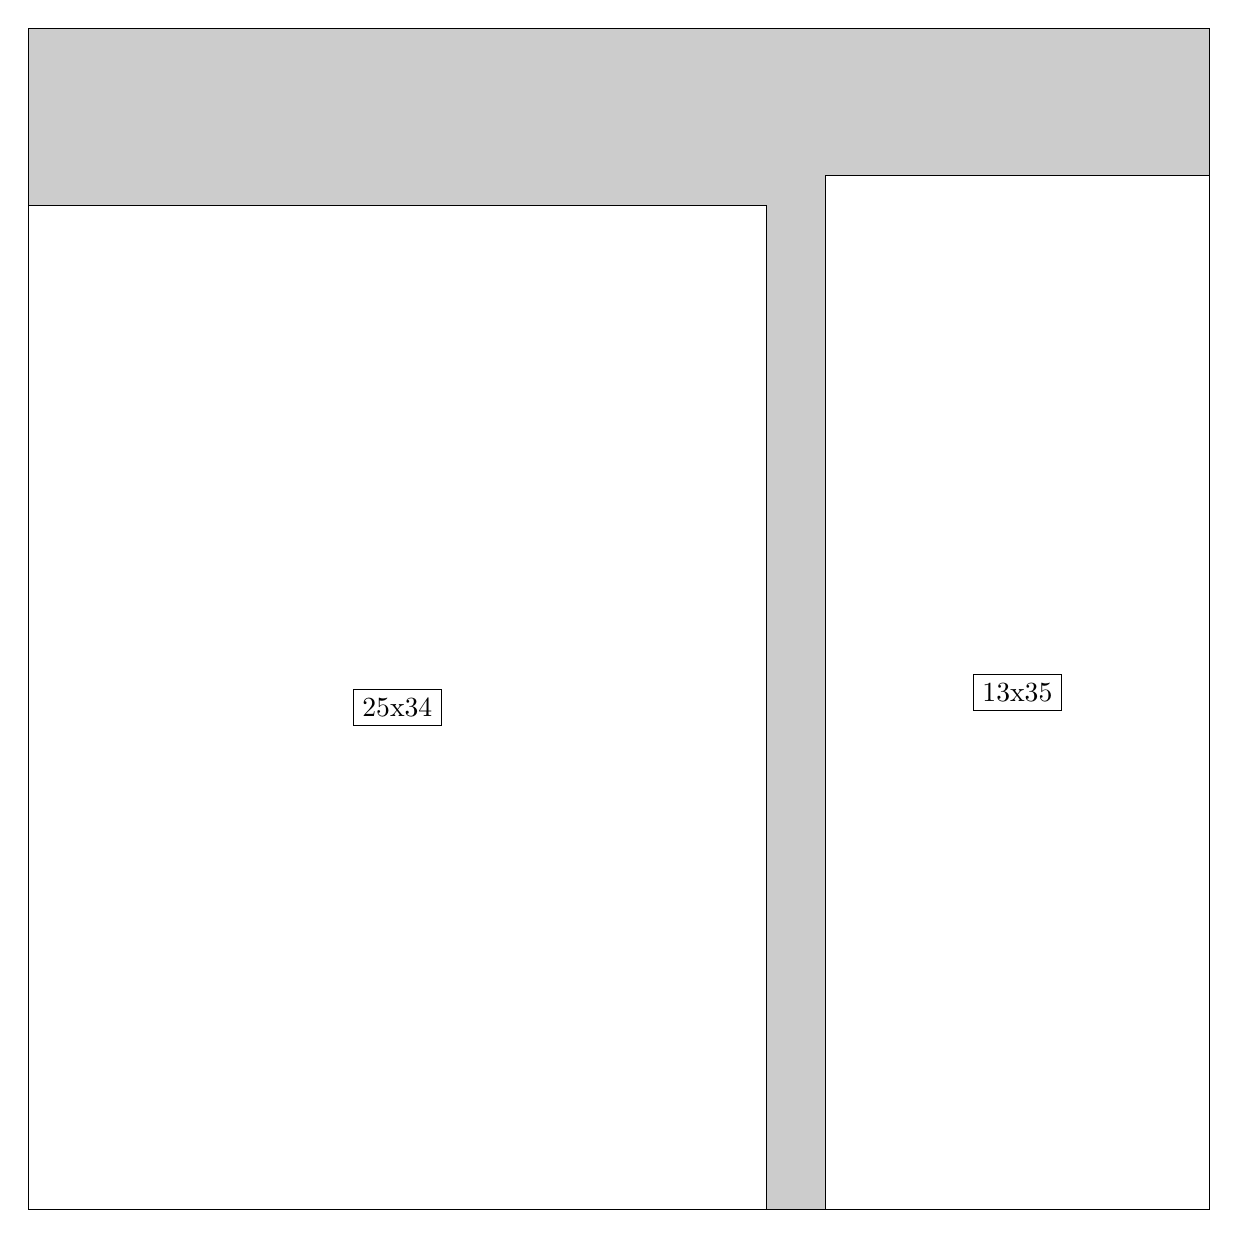
\begin{tikzpicture}[shorten >=1pt,scale=1.0,every node/.style={scale=1.0},->]
\tikzstyle{vertex}=[circle,fill=black!25,minimum size=14pt,inner sep=0pt]
\filldraw[fill=gray!40!white, draw=black] (0,0) rectangle (15.0,15.0);
\foreach \name/\x/\y/\w/\h in {13x35/10.125/0.0/4.875/13.125,25x34/0.0/0.0/9.375/12.75}
\filldraw[fill=white!40!white, draw=black] (\x,\y) rectangle node[draw] (\name) {\name} ++(\w,\h);
\end{tikzpicture}


w =13 , h =35 , x =27 , y =0 , v =455
\par
w =25 , h =34 , x =0 , y =0 , v =850
\par
\newpage


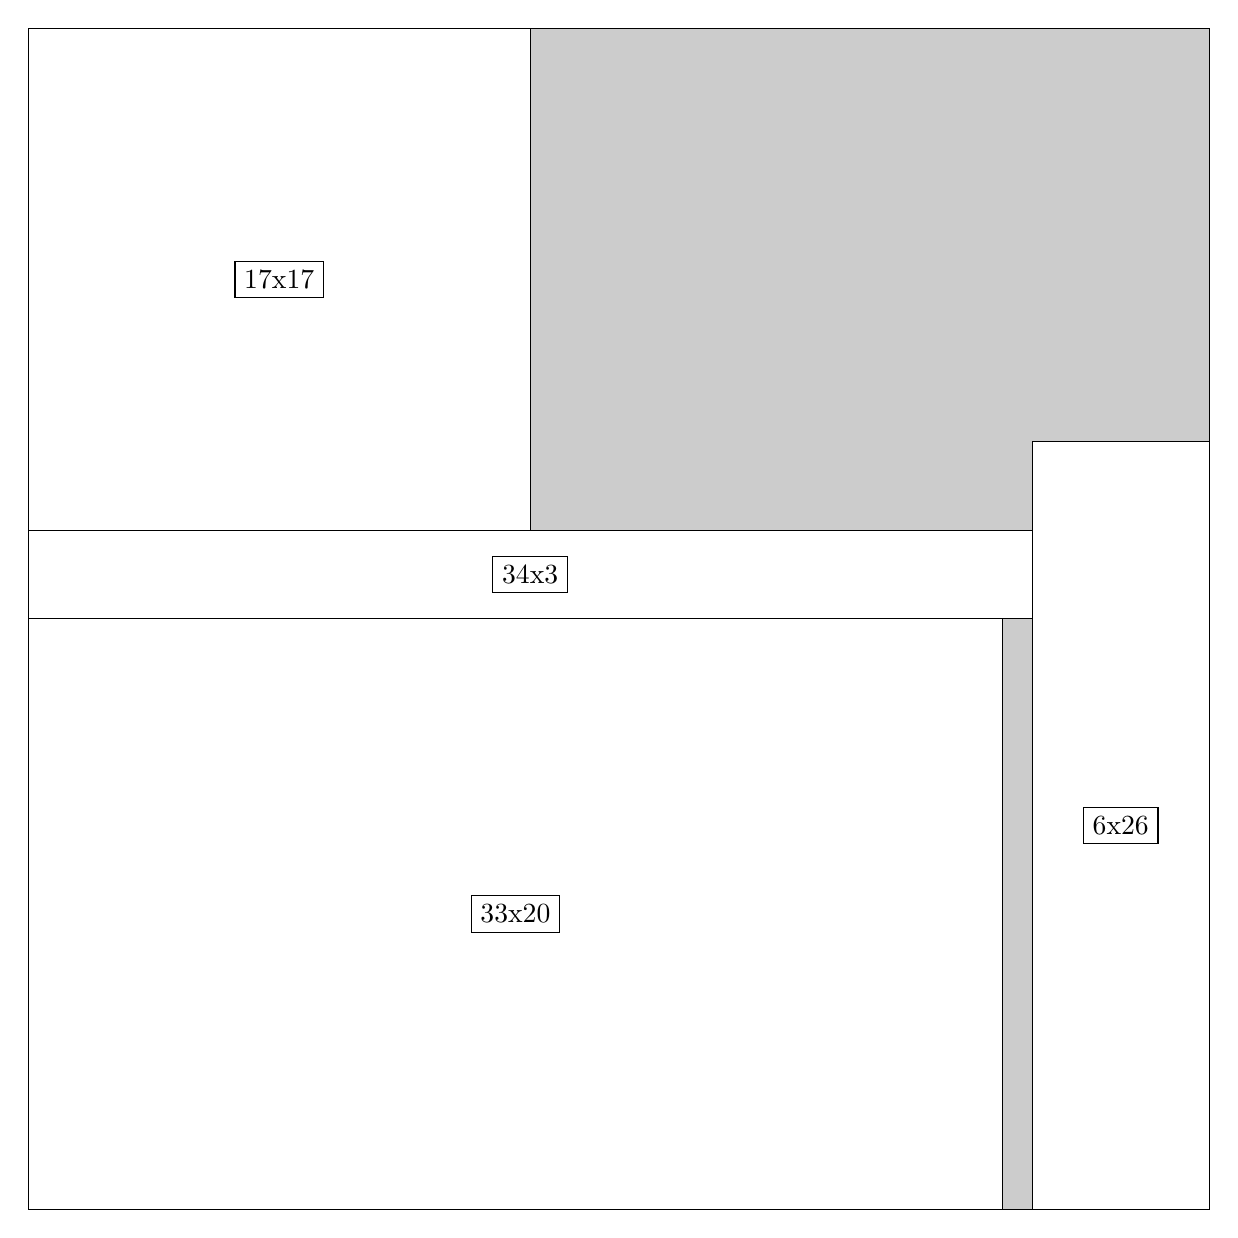
\begin{tikzpicture}[shorten >=1pt,scale=1.0,every node/.style={scale=1.0},->]
\tikzstyle{vertex}=[circle,fill=black!25,minimum size=14pt,inner sep=0pt]
\filldraw[fill=gray!40!white, draw=black] (0,0) rectangle (15.0,15.0);
\foreach \name/\x/\y/\w/\h in {33x20/0.0/0.0/12.375/7.5,17x17/0.0/8.625/6.375/6.375,6x26/12.75/0.0/2.25/9.75,34x3/0.0/7.5/12.75/1.125}
\filldraw[fill=white!40!white, draw=black] (\x,\y) rectangle node[draw] (\name) {\name} ++(\w,\h);
\end{tikzpicture}


w =33 , h =20 , x =0 , y =0 , v =660
\par
w =17 , h =17 , x =0 , y =23 , v =289
\par
w =6 , h =26 , x =34 , y =0 , v =156
\par
w =34 , h =3 , x =0 , y =20 , v =102
\par
\newpage


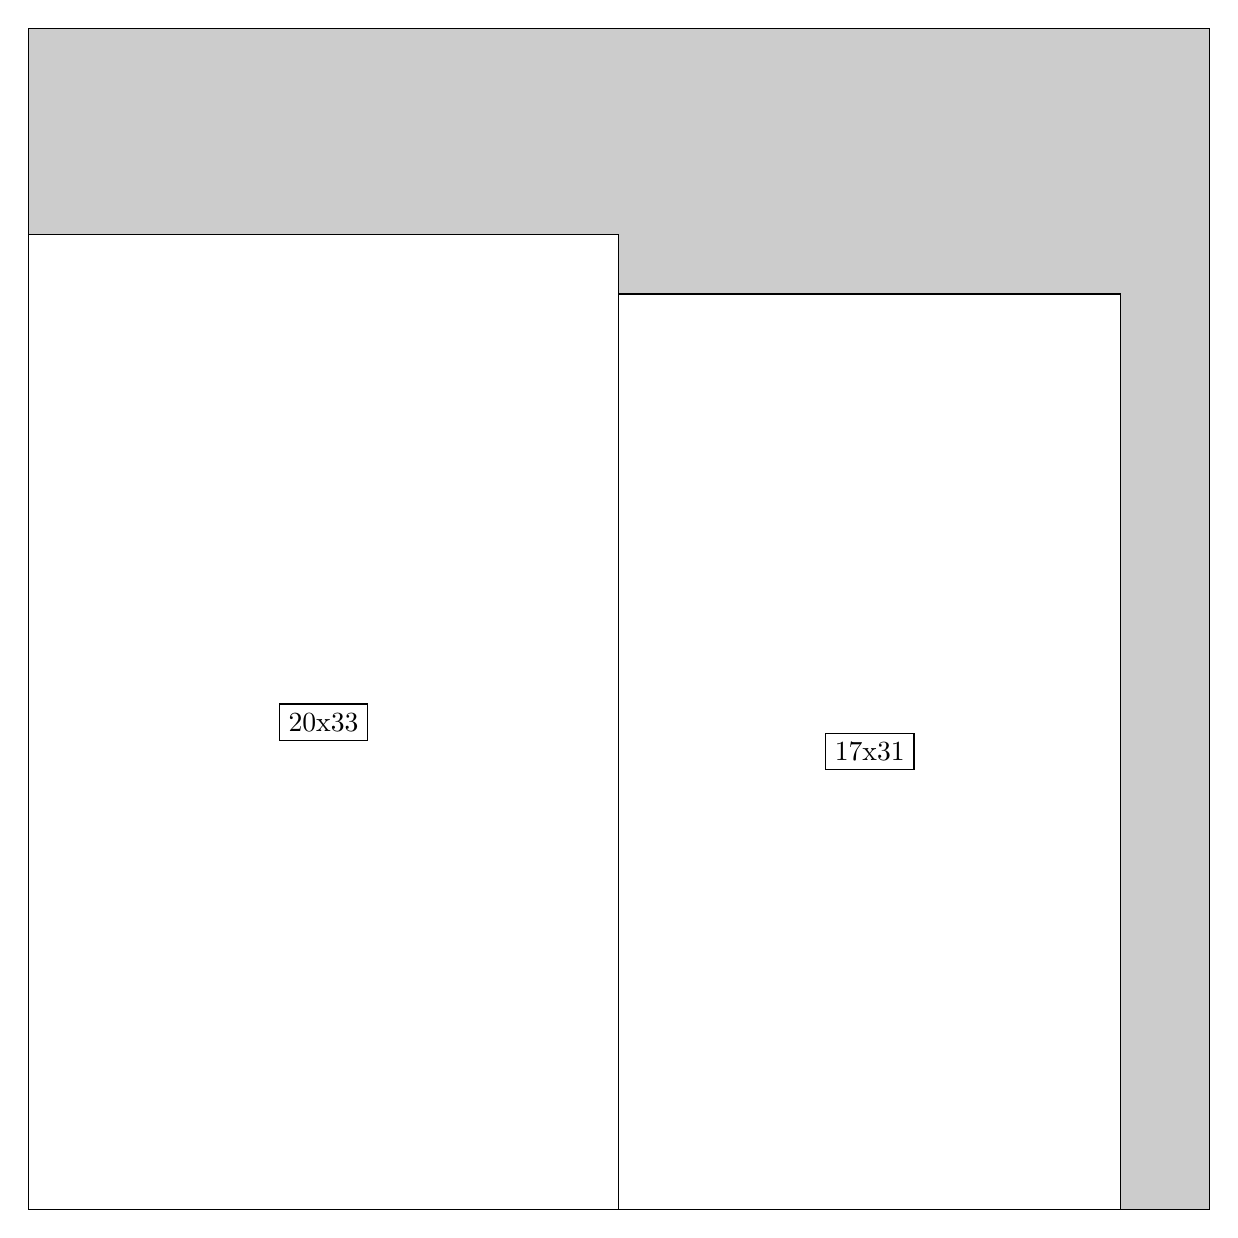
\begin{tikzpicture}[shorten >=1pt,scale=1.0,every node/.style={scale=1.0},->]
\tikzstyle{vertex}=[circle,fill=black!25,minimum size=14pt,inner sep=0pt]
\filldraw[fill=gray!40!white, draw=black] (0,0) rectangle (15.0,15.0);
\foreach \name/\x/\y/\w/\h in {20x33/0.0/0.0/7.5/12.375,17x31/7.5/0.0/6.375/11.625}
\filldraw[fill=white!40!white, draw=black] (\x,\y) rectangle node[draw] (\name) {\name} ++(\w,\h);
\end{tikzpicture}


w =20 , h =33 , x =0 , y =0 , v =660
\par
w =17 , h =31 , x =20 , y =0 , v =527
\par
\newpage


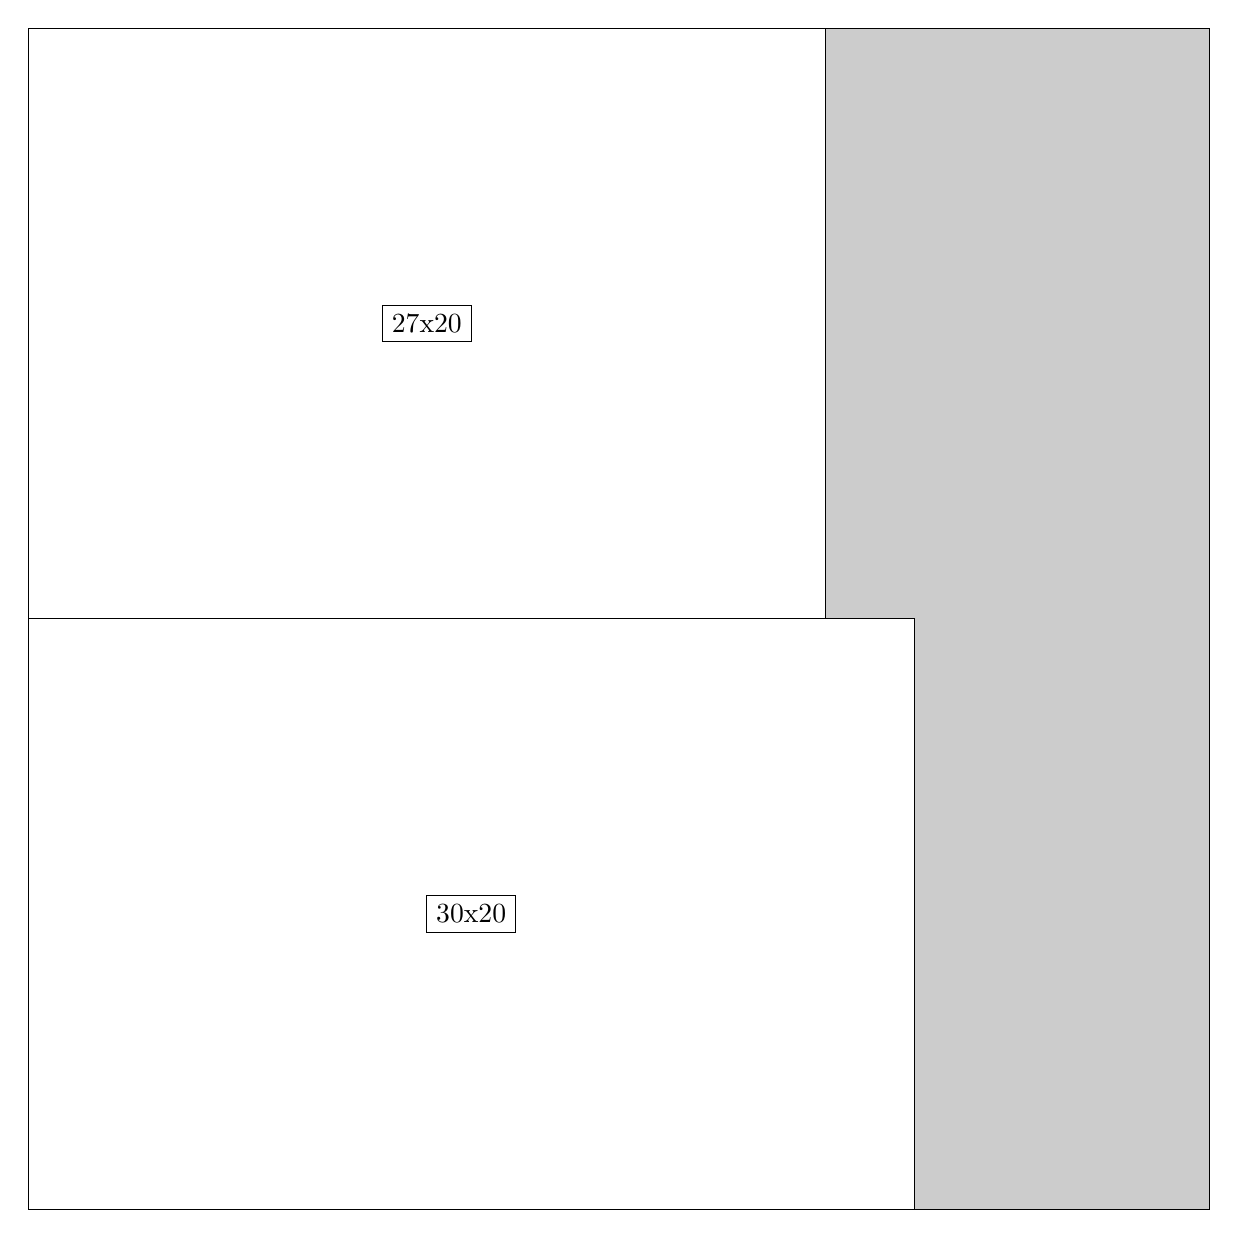
\begin{tikzpicture}[shorten >=1pt,scale=1.0,every node/.style={scale=1.0},->]
\tikzstyle{vertex}=[circle,fill=black!25,minimum size=14pt,inner sep=0pt]
\filldraw[fill=gray!40!white, draw=black] (0,0) rectangle (15.0,15.0);
\foreach \name/\x/\y/\w/\h in {30x20/0.0/0.0/11.25/7.5,27x20/0.0/7.5/10.125/7.5}
\filldraw[fill=white!40!white, draw=black] (\x,\y) rectangle node[draw] (\name) {\name} ++(\w,\h);
\end{tikzpicture}


w =30 , h =20 , x =0 , y =0 , v =600
\par
w =27 , h =20 , x =0 , y =20 , v =540
\par
\newpage


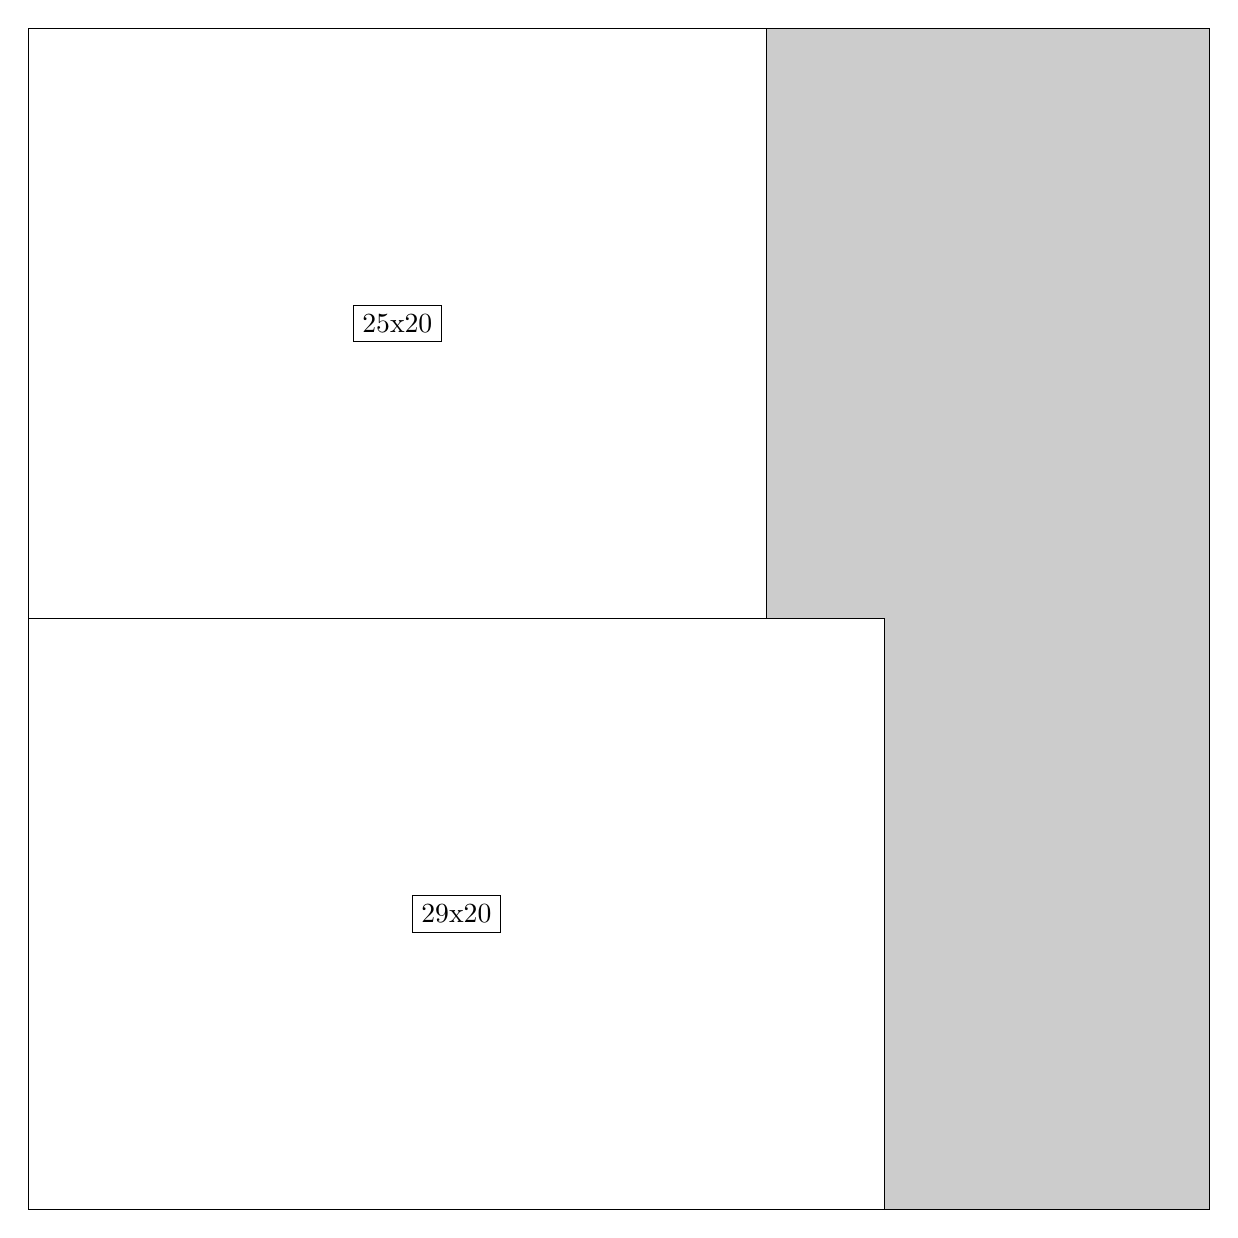
\begin{tikzpicture}[shorten >=1pt,scale=1.0,every node/.style={scale=1.0},->]
\tikzstyle{vertex}=[circle,fill=black!25,minimum size=14pt,inner sep=0pt]
\filldraw[fill=gray!40!white, draw=black] (0,0) rectangle (15.0,15.0);
\foreach \name/\x/\y/\w/\h in {29x20/0.0/0.0/10.875/7.5,25x20/0.0/7.5/9.375/7.5}
\filldraw[fill=white!40!white, draw=black] (\x,\y) rectangle node[draw] (\name) {\name} ++(\w,\h);
\end{tikzpicture}


w =29 , h =20 , x =0 , y =0 , v =580
\par
w =25 , h =20 , x =0 , y =20 , v =500
\par
\newpage


\end{document}